\documentclass[a4paper]{article}
\usepackage[utf8]{inputenc}
\usepackage[russian,english]{babel}
\usepackage[T2A]{fontenc}
\usepackage[left=10mm, top=20mm, right=18mm, bottom=15mm, footskip=10mm]{geometry}
\usepackage{indentfirst}
\usepackage{amsmath,amssymb}
\usepackage{mathastext} 
\usepackage[italicdiff]{physics}
\usepackage{graphicx}
\usepackage{caption}
\usepackage{float}
\usepackage{caption}
\renewcommand{\thefootnote}{\fnsymbol{footnote}}
\usepackage{tablefootnote}
\usepackage{footmisc}
\usepackage{textcomp}
\usepackage{multicol}
\usepackage[parfill]{parskip}
\usepackage{makecell}
\usepackage{array}  
\renewcommand\cellalign{cc} 
\renewcommand\cellgape{\Gape[2pt]} 
\usepackage[utf8]{inputenc}\newcommand{\approxtext}[1]{\ensuremath{\stackrel{\text{#1}}{\approx}}}
\usepackage[colorlinks=true, urlcolor=blue, linkcolor=blue, citecolor=blue]{hyperref}
\graphicspath{{images/}}
\DeclareGraphicsExtensions{.pdf,.png,.jpg}
\usepackage{wrapfig}
\captionsetup{labelformat=empty}
\usepackage{caption}
\captionsetup[figure]{name=Рисунок}
\captionsetup[table]{name=Таблица}
  
\title{\textbf{Отчет о выполнении лабораторной работы 3.6.1}}
\date{}
\author{Котляров Михаил, Б01-402}

\begin{document}

\maketitle
	
	\section{Введение}
	
	\textbf{Цель работы:} изучить спектры сигналов различной формы и влияние параметров сигнала на вид соответствующих спектров; проверить справедливость соотношений неопределённостей;\\

	\textbf{Оборудование:} генератор сигналов произвольной формы, цифровой осциллограф с функцией быстрого преобразования Фурье или цифровой USB-осциллограф, подключённый к персональному компьютеру.
	
	\section{Теоретические сведения}

Согласно теореме Фурье, любая периодическая функция может быть представлена в виде ряда (конечного или бесконечного) гармонических функций с кратными частотами — ряда Фурье. Одно из представлений ряда Фурье для функции с периодом $T$ имеет вид:

\begin{equation}
f(t) = \dfrac{a_0}{2} + \sum\limits_{n = 1}^{\infty}\left[a_n \cos \left(n \omega_0t + \varphi_0\right) + b_n \sin \left(n \omega_0t + \varphi_0\right)\right],
\end{equation}
или 
\begin{equation}
f(t) = \dfrac{a_0}{2} + \sum\limits_{n = 1}^{\infty}A_n \cos \left(n\omega_0t-\varphi_n\right).
\end{equation}
Коэффициенты определяются следующим образом:
\begin{align}
c_n &= \displaystyle \frac{1}{T} \int_0^Tf(t)e^{-in\omega_0t} \, dt, & A_n &= 2\abs{c_n} = \sqrt{a_n^2 + b_n^2}, & \varphi_n = arg\, c_n = \arctan{\frac{b_n}{a_n}}.
\end{align}

Совокупность всех частот $\nu_n = \frac{\omega_n}{2\pi}$ и соответствующих им амплитуд $A_n$ называется спектром функции $f(t)$.
Пусть $\Delta t$ - характерное время $f(t)$ (период, длительность импульса и т.п), $\Delta \nu$ - характерный масштаб частоты, тогда справедливо \textit{соотношение неопределенностей}:
\begin{equation}
\Delta \nu_n \cdot \Delta t \sim 1.
\end{equation}

\section*{Теорема смещения}

Найдём спектр $F(\omega)$ сигнала, смещённого по времени: $f(t) = f_0(t - \tau)$, где $f_0(t)$ — функция с известным спектром $F_0(\omega) = \mathcal{F}[f_0]$.

По определению имеем
\begin{equation}
F(\omega) = \mathcal{F}[f(t)] = \int_{-\infty}^{\infty} f_0(t - \tau) e^{-i\omega t}\, dt.
\end{equation}

После замены переменных $t' = t - \tau$ ($dt = dt'$) получаем
\begin{equation}
F(\omega) = \int_{-\infty}^{\infty} f_0(t') e^{-i\omega(t' + \tau)}\, dt'.
\end{equation}

Множитель $e^{-i\omega\tau}$ (не зависящий от переменной интегрирования $t'$) выносится из-под знака интеграла:
\begin{equation}
F(\omega) = e^{-i\omega\tau} \int_{-\infty}^{\infty} f_0(t') e^{-i\omega t'}\, dt' = e^{-i\omega\tau} \cdot F_0(\omega),
\end{equation}
или символически
\begin{equation}
\mathcal{F}[f_0(t - \tau)] = e^{-i\omega\tau} \mathcal{F}[f_0(t)],
\end{equation}

т.е. смещение сигнала во времени на $\tau$ (запаздывание) приводит к умножению его спектра на $e^{-i\omega\tau}$ (теорема смещения).

Заметим, что поскольку $|e^{-i\omega\tau}| = 1$, смещение по времени не меняет амплитуд спектральных компонент, а лишь сдвигает их фазы (пропорционально частоте компоненты).

\subsection*{Амплитудная модуляция}

Модулированный сигнал:
\begin{equation}
f_{\text{AM}}(t) = a_0 \left(1 + m \cos(\Omega t)\right) \cos(\omega_0 t), \quad 0 < m \leq 1.
\end{equation}

Раскрывая произведение, получаем:
\begin{equation}
f_{\text{AM}}(t) = a_0 \cos(\omega_0 t) + \frac{m a_0}{2} \cos\left((\omega_0 - \Omega)t\right) + \frac{m a_0}{2} \cos\left((\omega_0 + \Omega)t\right).
\end{equation}

Спектр состоит из трёх гармоник:
\begin{enumerate}
\item Несущая: частота $\omega_0$, амплитуда $a_0$, фаза $0$;
\item Две боковые: частоты $\omega_0 - \Omega$, $\omega_0 + \Omega$,  амплитуда $\frac{m a_0}{2}$, фаза $0$.
\end{enumerate}

Все компоненты находятся в фазе.
\subsection*{Фазовая модуляция}

Модулированный сигнал:
\begin{equation}
f_{\text{FM}}(t) = a_0 \cos\left(\omega_0 t + m \cos(\Omega t)\right).
\end{equation}

При малой глубине модуляции ($m \ll 1$) используется приближение:
\begin{equation}
f_{\text{FM}}(t) \approx a_0 \cos(\omega_0 t) + \frac{m a_0}{2} \cos\left((\omega_0 - \Omega)t + \frac{\pi}{2}\right) + \frac{m a_0}{2} \cos\left((\omega_0 + \Omega)t + \frac{\pi}{2}\right).
\end{equation}

Спектр состоит из трёх гармоник:
\begin{enumerate}
\item Несущая: частота $\omega_0$, амплитуда $a_0$, фаза $0$;
   \item две боковые: частота частоты $\omega_0 - \Omega$, $\omega_0 + \Omega$, амплитуда $\frac{m a_0}{2}$, фаза $\frac{\pi}{2}$;
\end{enumerate}

При большой глубине модуляции ($m \gg 1$) спектр расширяется. Сигнал выражается через ряд:
\begin{equation}
f_{\text{FM}}(t) = a_0 \sum_{n=-\infty}^{\infty} J_n(m) \cos\left((\omega_0 + n\Omega)t\right),
\end{equation}
где $J_n(m)$ — функции Бесселя первого рода порядка $n$, определяется как коэффициенты разложения в ряд Фурье функции $e^{i m \cos \theta}$:
\begin{equation}
e^{i m \cos \theta} = \sum_{n=-\infty}^{\infty} i^n J_n(m) e^{i n \theta},
\end{equation}
или, эквивалентно, интегральным представлением:
\begin{equation}
J_n(m) = \frac{1}{2\pi} \int_{-\pi}^{\pi} \cos(n\theta - m \sin\theta)\, d\theta.
\end{equation}

Они также являются решениями дифференциального уравнения Бесселя:
\begin{equation}
x^2 \frac{d^2 y}{dx^2} + x \frac{dy}{dx} + (x^2 - n^2)y = 0.
\end{equation}

Для целых $n$ функции $J_n(m)$ вещественны при вещественном $m$ и описывают амплитуды спектральных компонент при фазовой и частотной модуляции.
Появляются дополнительные боковые компоненты с частотами $\omega_0 \pm n\Omega$, $n = 1,2,3,\dots$.

\section{Выполнение}
\begin{enumerate}
\subsection{А. Исследование спектра периодической последовательности
прямоугольных импульсов и проверка соотношений неопределённостей}
\item Настроим генерацию прямоугольных импульсов с рекомендованными параметрами: частота повторения $\nu_{\text{повт}} = 1$ кГц (период $T = \frac{1}{\nu_{\text{повт}}}$ = 1 мс), и длительность импульса $\tau = \frac{T}{20}$ = 50 мкс.
Далее: а) при фиксированной длительности импульса меняем $\nu_{\text{повт}}$; б) фиксируем $\nu_{\text{повт}}$ и меняем $\tau$.

\begin{figure}[h!]
\centering

% Строка 1
\begin{minipage}{0.48\textwidth}
  \centering
  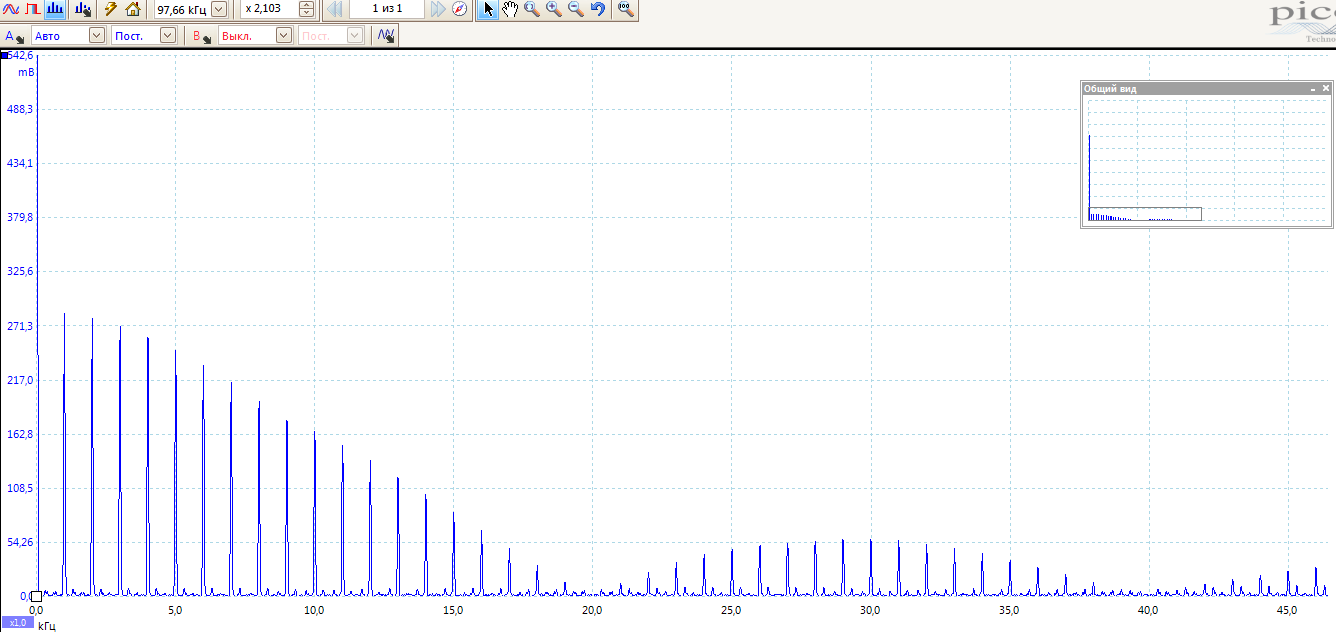
\includegraphics[width=\linewidth]{Graphics/A_1_50.PNG}
  \caption{График 1. $\nu_{\text{повт}} = 1$ кГц, $\tau = 50$ мкс.}
\end{minipage}
\hfill
\begin{minipage}{0.48\textwidth}
  \centering
  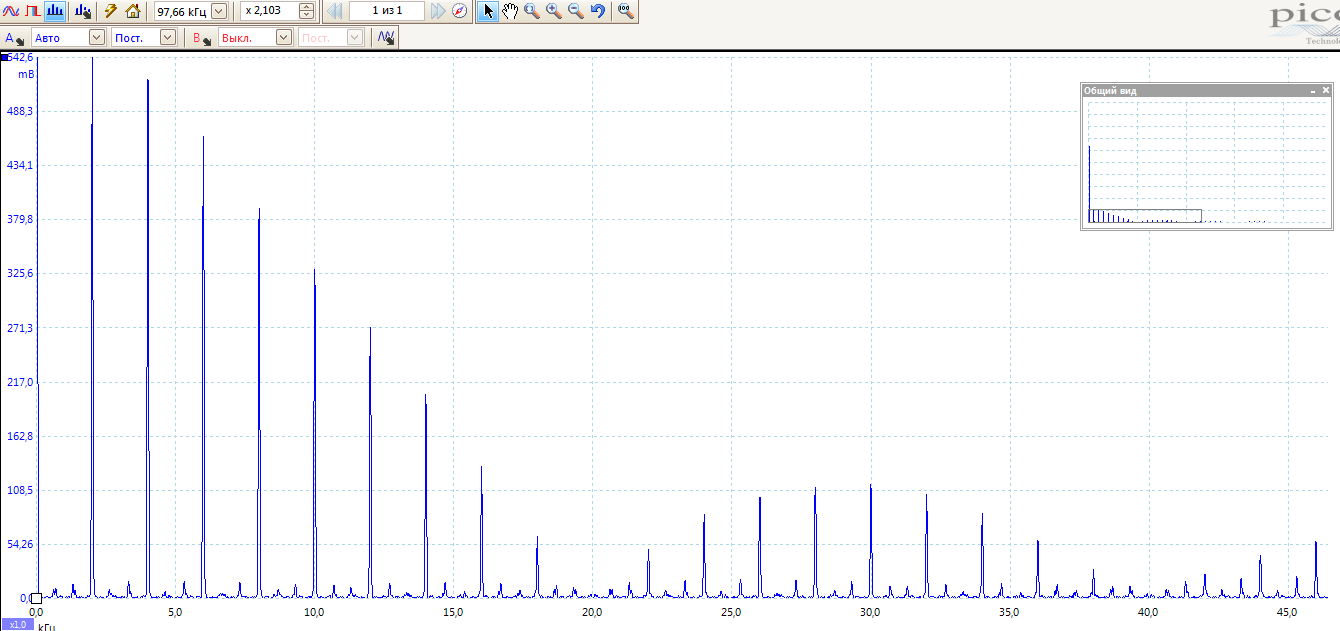
\includegraphics[width=\linewidth]{Graphics/A_2_50.PNG}
  \caption{График 2. $\nu_{\text{повт}} = 2$ кГц, $\tau = 50$ мкс.}
\end{minipage}

\vspace{1em} % Отступ между строками

% Строка 2
\begin{minipage}{0.48\textwidth}
  \centering
  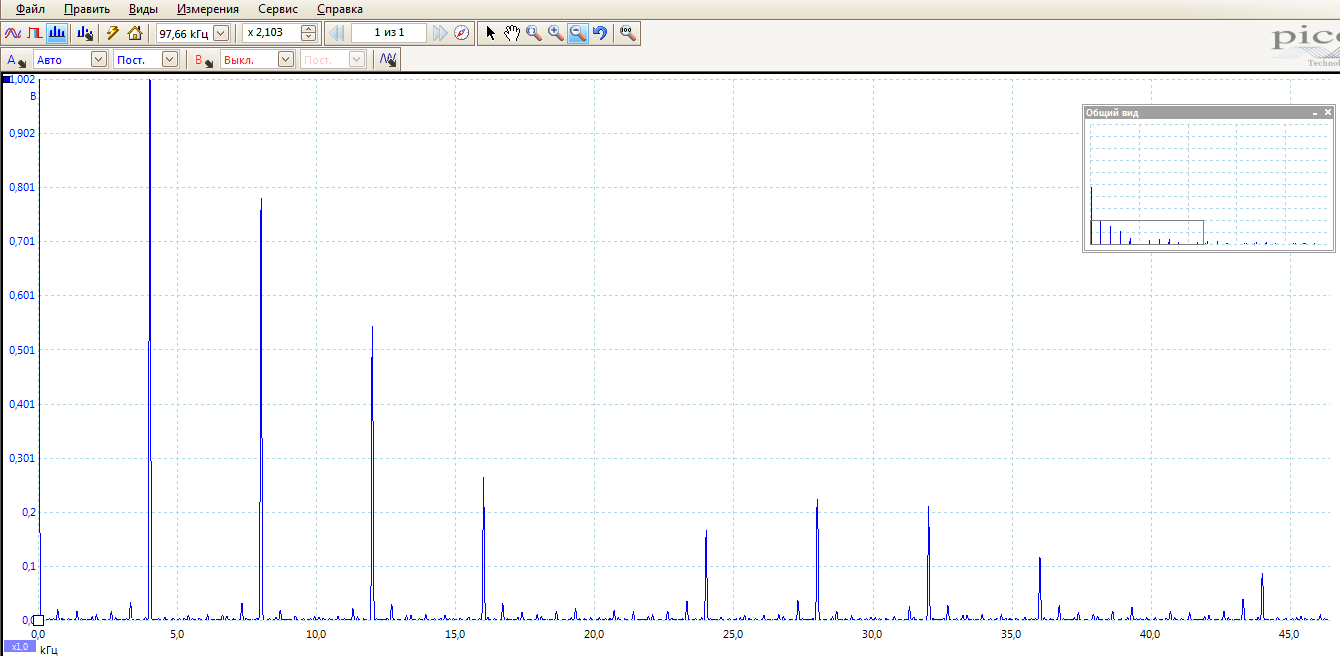
\includegraphics[width=\linewidth]{Graphics/A_4_50.PNG}
  \caption{График 3. $\nu_{\text{повт}} = 4$ кГц, $\tau = 50$ мкс.}
\end{minipage}
\hfill
\begin{minipage}{0.48\textwidth}
  \centering
  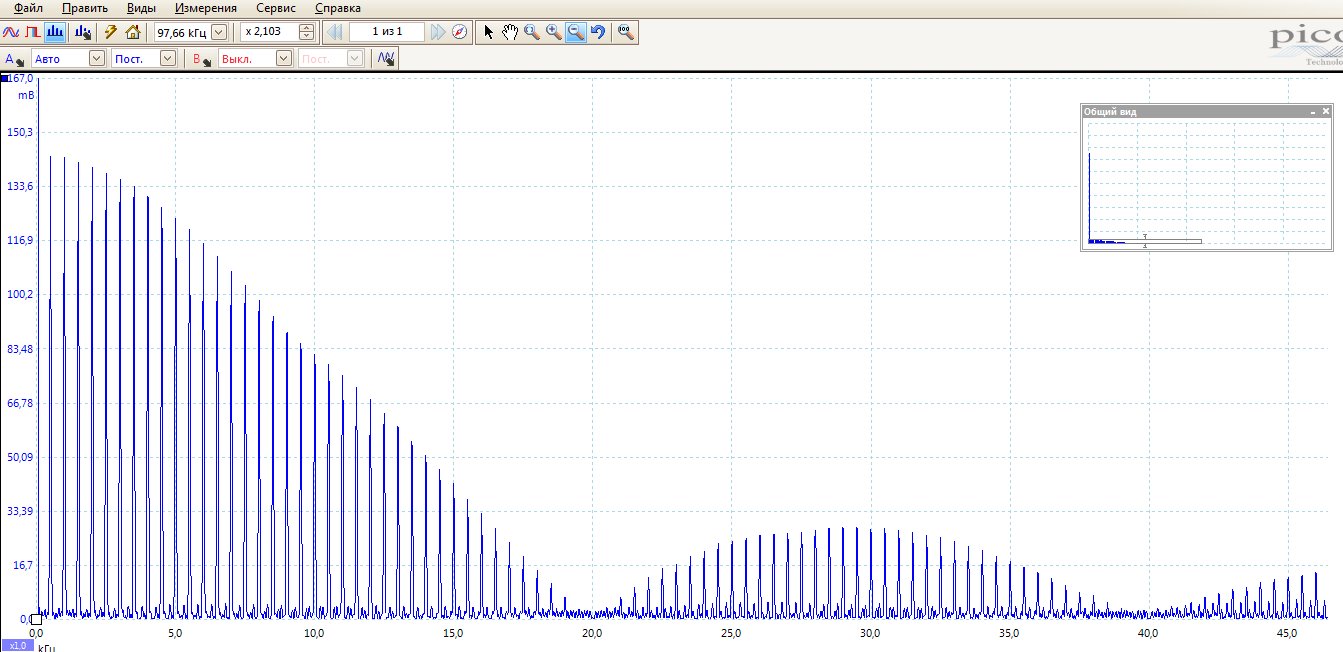
\includegraphics[width=\linewidth]{Graphics/A_05_50.PNG}
  \caption{График 4. $\nu_{\text{повт}} = 0{,}5$ кГц, $\tau = 50$ мкс.}
\end{minipage}

\vspace{1em}

% Строка 3
\begin{minipage}{0.48\textwidth}
  \centering
  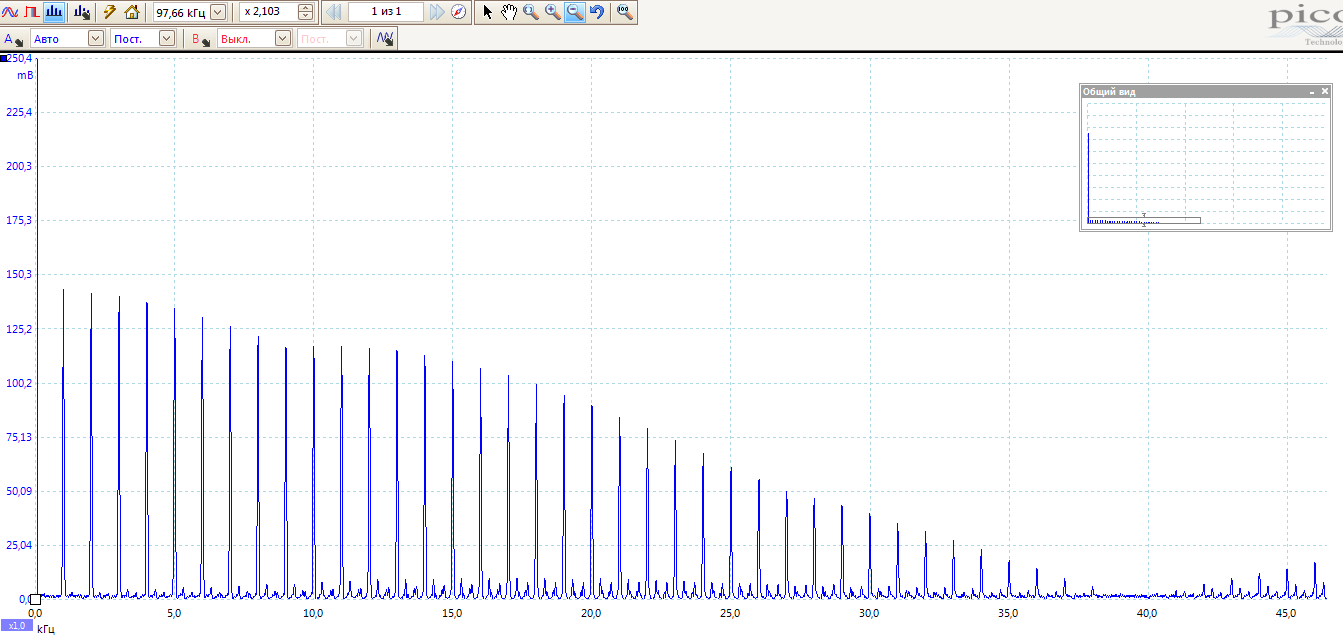
\includegraphics[width=\linewidth]{Graphics/A_1_25.PNG}
  \caption{График 5. $\nu_{\text{повт}} = 1$ кГц, $\tau = 25$ мкс.}
\end{minipage}
\hfill
\begin{minipage}{0.48\textwidth}
  \centering
  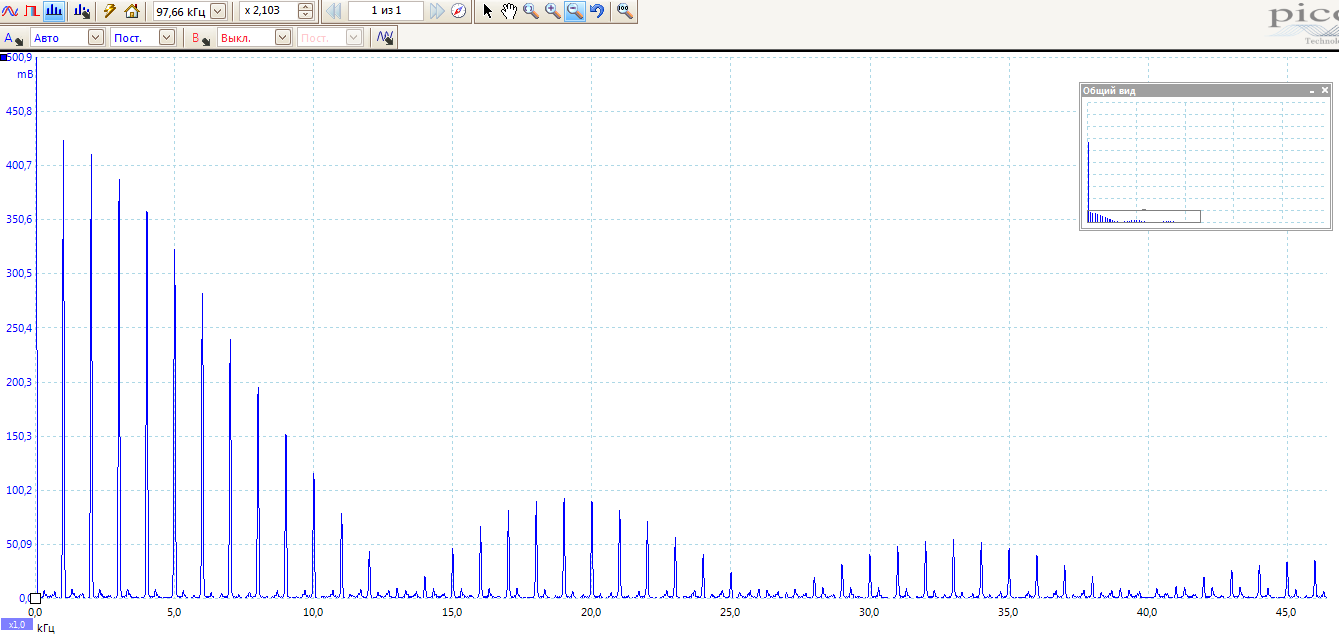
\includegraphics[width=\linewidth]{Graphics/A_1_75.PNG}
  \caption{График 6. $\nu_{\text{повт}} = 1$ кГц, $\tau = 75$ мкс.}
\end{minipage}

\vspace{1em}

% Строка 4 (один график — можно центрировать)
\begin{minipage}{0.48\textwidth}
  \centering
  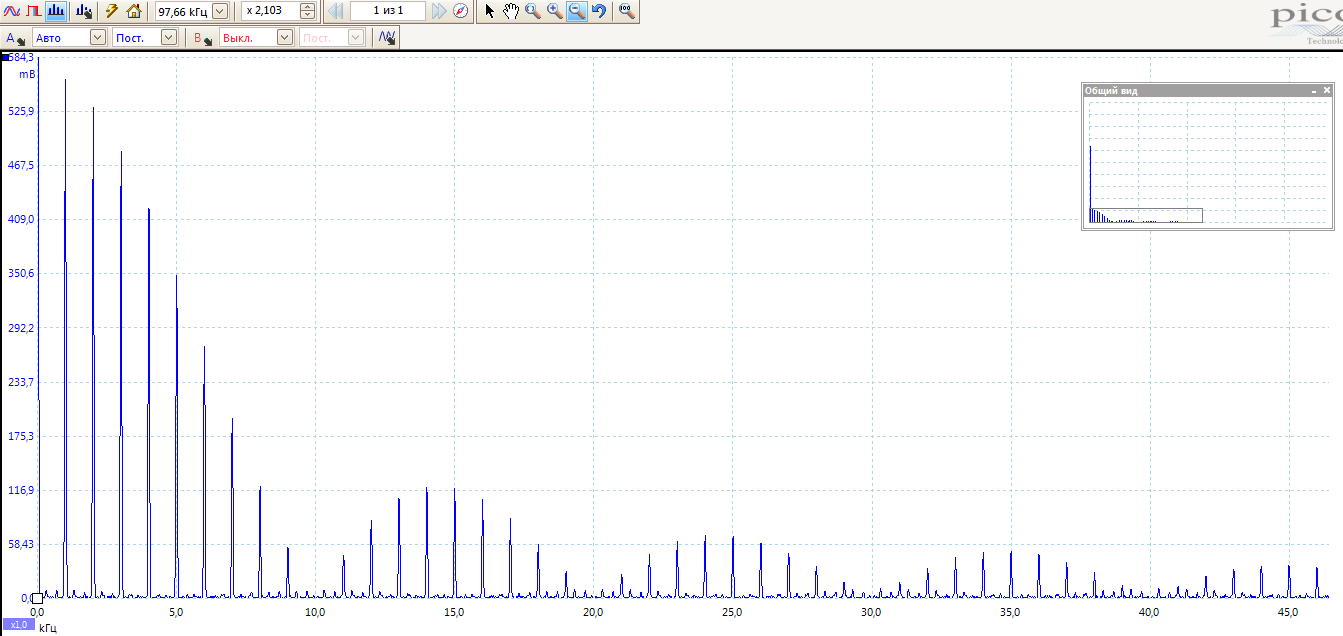
\includegraphics[width=\linewidth]{Graphics/A_1_100.PNG}
  \caption{График 7. $\nu_{\text{повт}} = 1$ кГц, $\tau = 100$ мкс.}
\end{minipage}

\end{figure}

Как мы видим, с увеличением длительности импульса $\tau$ уменьшается ширина спектра, с увеличением периода (уменьшением частоты повторений), уменьшается расстояние между гармониками. Это отражает достоверность соотношения неопределенностей.

\item При фиксированных рекомендованных параметрах измерим амплитуды и частоты первых 8 гармоник, начиная с первой и сравним с теоретическими: $\nu_n = n \cdot \nu_{\text{повт}}$, $\abs{a_n} = \frac{\abs{\sin{\frac{\pi n \tau}{T}}}}{\pi n}$.
\begin{table}[h!]
    \centering
    \begin{tabular}{|c|c|c|c|c|c|c|c|c|}
        \hline
        $n$ & 1 & 2 & 3 & 4 & 5 & 6 & 7 & 8 \\ \hline
        $\nu_n^{\text{теор}},\ \text{кГц}$ & 1{,}04 & 2{,}004 & 3{,}017 & 3{,}988 & 4{,}994 & 6{,}001 & 7{,}008 & 7{,}978 \\ \hline
        $\nu_n^{\text{эксп}},\ \text{кГц}$ & 1 & 2 & 3 & 4 & 5 & 6 & 7 & 8 \\  \hline
        $|a_n|^{\text{эксп}},\ \text{мВ}$ & 283{,}3 & 278{,}1 & 272{,}2 & 260{,}4 & 246{,}5 & 231{,}2 & 213{,}9 & 195{,}1 \\ \hline
        $\left|\frac{a_n}{a_1}\right|^{\text{эксп}}$ & 1 & 0{,}9816 & 0{,}9608 & 0{,}9192 & 0{,}8701 & 0{,}8161 & 0{,}7550 & 0{,}6887 \\ \hline
        $\left|\frac{a_n}{a_1}\right|^{\text{теор}}$ & 1 & 0{,}9877 & 0{,}9674 & 0{,}9393 & 0{,}9040 & 0{,}8619 & 0{,}8137 & 0{,}7599 \\ \hline
    \end{tabular}
    \caption{Таблица 1. Сравнение теоретических и экспериментальных значений частоты и амплитуд гармоник.}
    \label{tab:spectra}
\end{table}

\item Далее зафиксируем период $T$, равный 1 мс, и будем менять длительность импульса в пределах от $\frac{T}{50}$, до $\frac{T}{5}$, измеряя ширину спектра $\Delta \nu$.

\begin{table}[h!]
    \centering
    \begin{tabular}{|c|c|c|c|c|c|c|c|}
        \hline
        $\tau,\ \text{мкс}$ & 20 & 25 & 40 & 75 & 100 & 150 & 200 \\
        \hline
        $\Delta \nu,\ \text{кГц}$ & 49{,}71 & 40{,}18 & 25{,}03 & 13{,}36 & 10{,}07 & 6{,}629 & 5{,}079 \\
        \hline
    \end{tabular}
    \caption{Таблица 2. Зависимость ширины спектра $\Delta \nu$ от длительности импульса $\tau$ при  $T = 1$ мс.}
    \label{tab:delta_nu_vs_tau}
\end{table}

По МНК построим график $\Delta \nu(\frac{1}{\tau})$.

\begin{figure}[h]
        \center{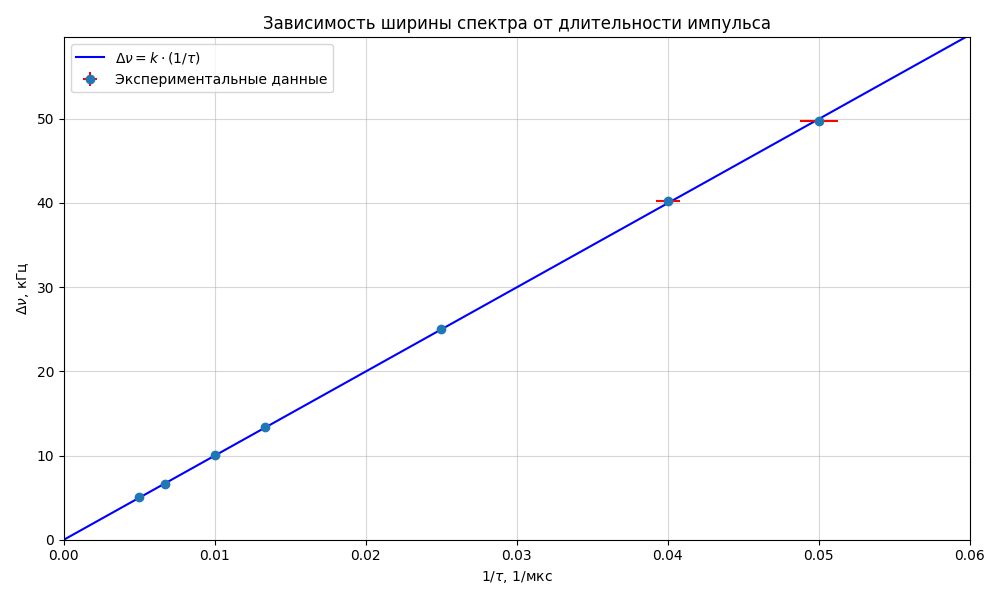
\includegraphics[width=1\textwidth]{Graphics/Delta_nu_vs_inv_tau_plot_A.png}}
        \caption{График 8. Зависимость ширины спектра от длительности импульса.}
\end{figure}

Наклон прямой $k = 0,99895 \pm 0,00004$ Гц$\cdot$с ($\varepsilon_k = 0,0037\%$). Таким образом, соотношение неопределенностей выполняется с высокой точностью.

\item Зафиксируем длительность импульса $\tau = 100$ мкс и будем менять период $T$ в пределах от $2\tau$ до $50 \tau$, измеряя расстояние между гармониками $\delta \nu = \nu_{n+1} - \nu_n$.

\clearpage
\begin{table}[h!]
    \centering
    \begin{tabular}{|c|c|c|c|c|c|c|c|}
        \hline
        $T,\ \text{мкс}$ & 200 & 500 & 1000 & 2000 & 3000 & 4000 & 5000 \\
        \hline
        $\delta \nu,\ \text{кГц}$ & 9{,}959 & 1{,}984 & 0{,}964 & 0{,}501 & 0{,}34 & 0{,}246 & 0{,}198 \\
        \hline
    \end{tabular}
    \caption{Таблица 3. Зависимость расстояния между гармониками $\delta \nu$ \\от периода $T$ при $\tau = 100$ мкс.}
    \label{tab:delta_nu_vs_T}
\end{table}

По МНК построим график $\delta \nu(\frac{1}{T})$.

\begin{figure}[h]
        \center{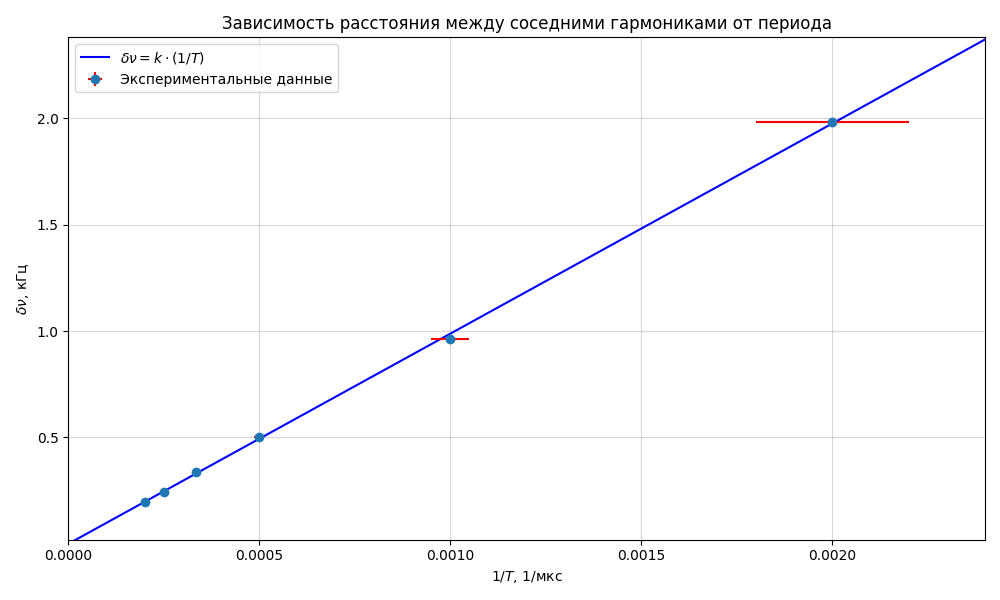
\includegraphics[width=1\textwidth]{Graphics/delta_nu_vs_inv_T_plot_G.png}}
        \caption{График 9. Зависимость расстояния между гармониками от периода.}
\end{figure}

Наклон прямой $k = 0,988 \pm 0,001$ Гц$\cdot$с ($\varepsilon_k = 0,11\%$). Как мы видим, соотношение неопределенностей выполняется с большой точностью.

\subsection{Б. Наблюдение спектра периодической последовательности цугов}
\item Установим режим подачи периодических импульсов синусоидальной формы («цугов») с рекомендованными параметрами: частота несущей $\nu_0 = 50$ кГц, период повторения $T = \frac{1}{\nu_{\text{повт}}}$ = 1 мс ($\nu_{\text{повт}} = 1$ кГц), число периодов синусоиды в одном импульсе $N = 5$ (что соответствует длительности импульса $\tau = \frac{N}{\nu_0} = 100$ мкс).\\
Будем менять каждый параметр при других фиксированных и измерять положение центра спектра, его ширину и расстояние между гармониками.

\clearpage
\begin{figure}[h!]
\centering

% Строка 1
\begin{minipage}{0.48\textwidth}
  \centering
  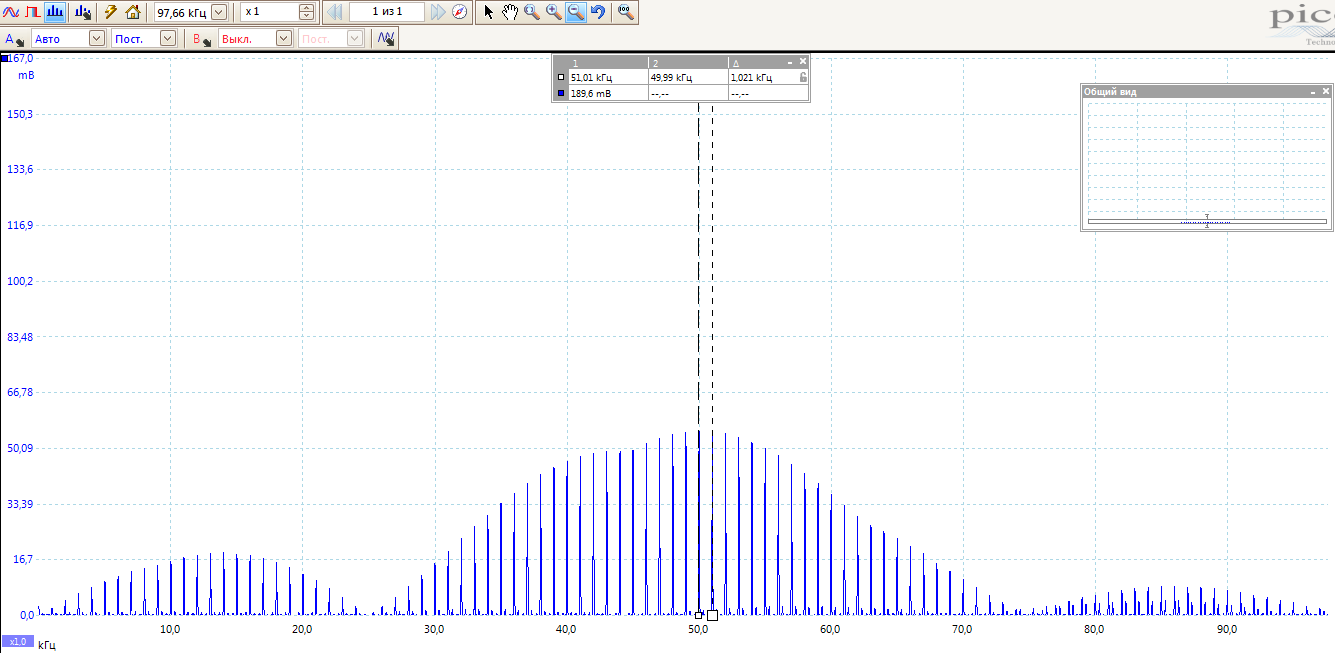
\includegraphics[width=\linewidth]{Graphics/Б_50_1_2.PNG}
  \caption{График 10. $\nu_0 = 50$ кГц, $T = 1$ мс, $N = 2$.}
\end{minipage}
\hfill
\begin{minipage}{0.48\textwidth}
  \centering
  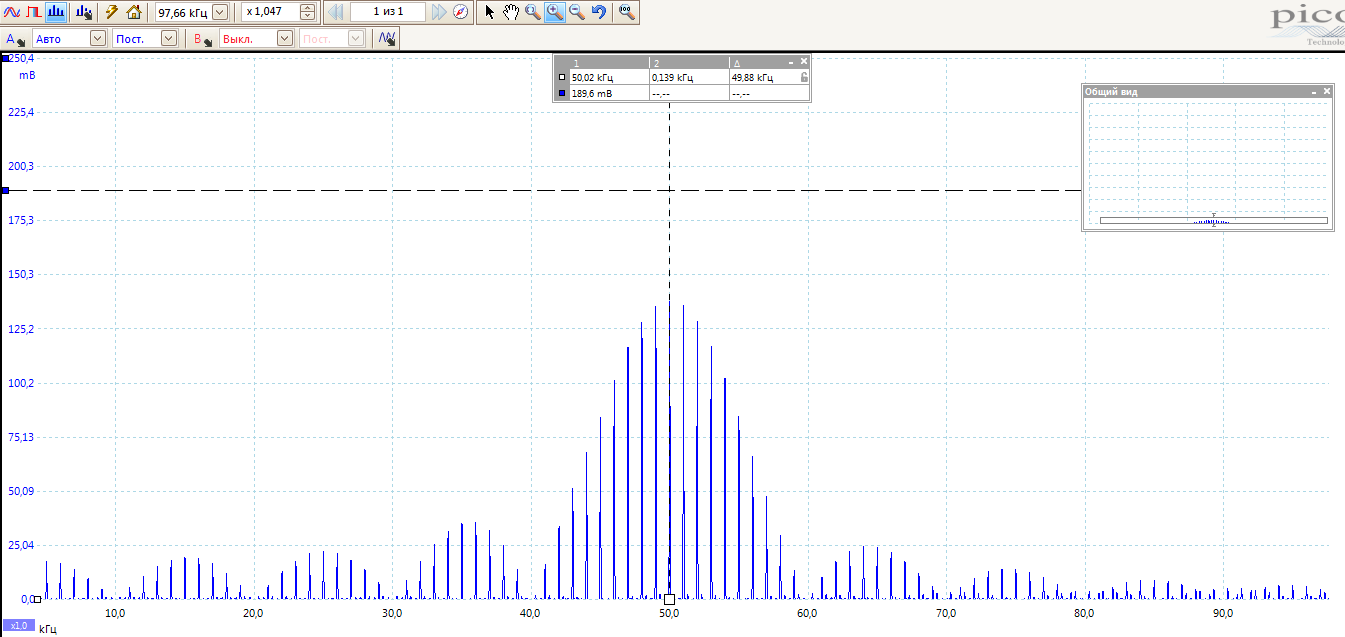
\includegraphics[width=\linewidth]{Graphics/Б_50_1_5.PNG}
  \caption{График 11. $\nu_0 = 50$ кГц, $T = 1$ мс, $N = 5$.}
\end{minipage}

\vspace{1em} % Отступ между строками

% Строка 2
\begin{minipage}{0.48\textwidth}
  \centering
  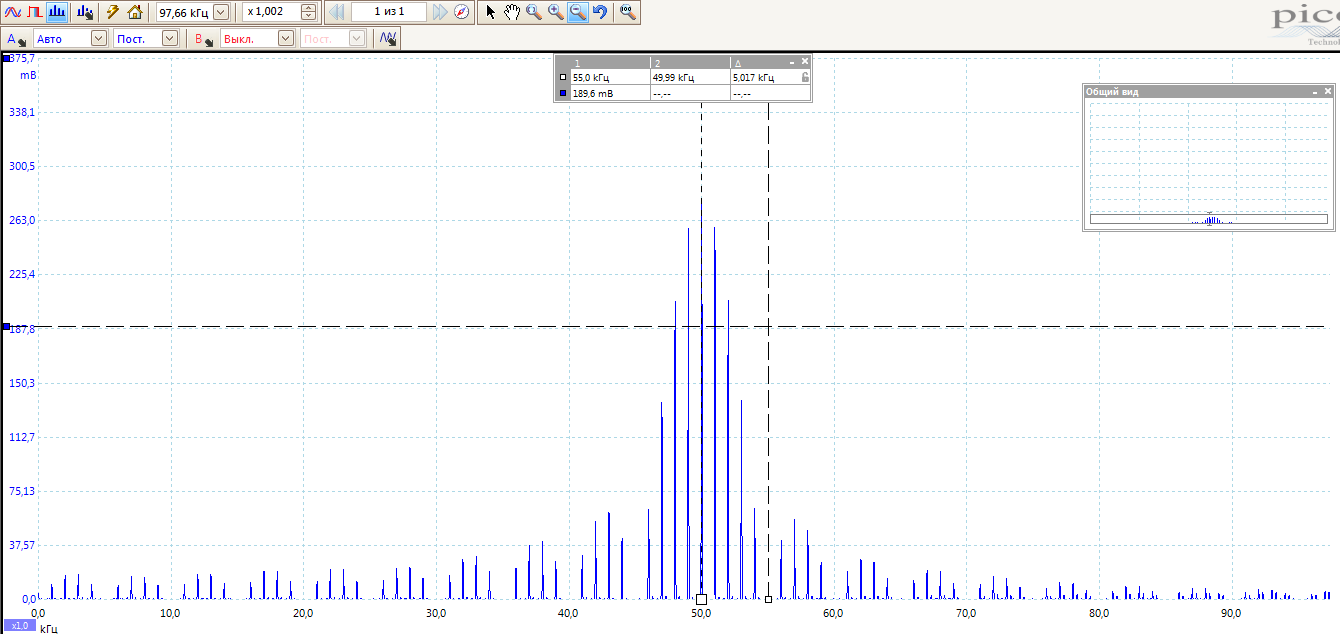
\includegraphics[width=\linewidth]{Graphics/Б_50_1_10.PNG}
  \caption{График 12. $\nu_0 = 50$ кГц, $T = 1$ мс, $N = 10$.}
\end{minipage}
\hfill
\begin{minipage}{0.48\textwidth}
  \centering
  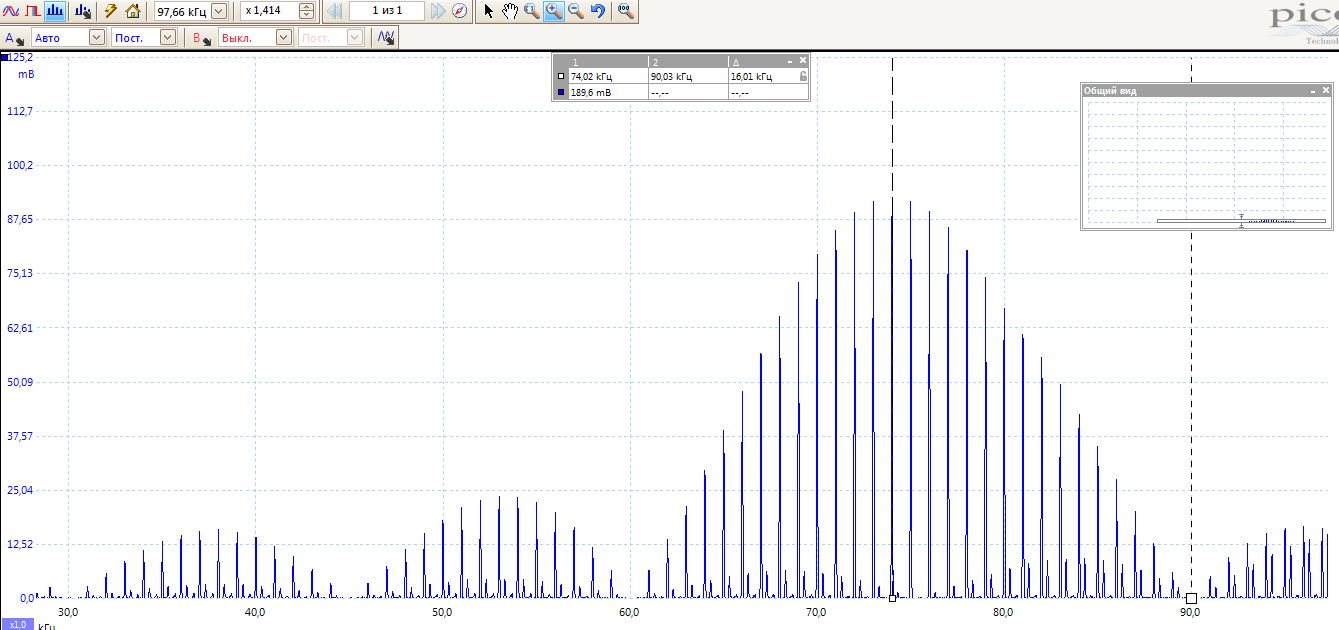
\includegraphics[width=\linewidth]{Graphics/Б_75_1_5.PNG}
  \caption{График 13. $\nu_0 = 75$ кГц, $T = 1$ мс, $N = 5$.}
\end{minipage}

\vspace{1em}

% Строка 3
\begin{minipage}{0.48\textwidth}
  \centering
  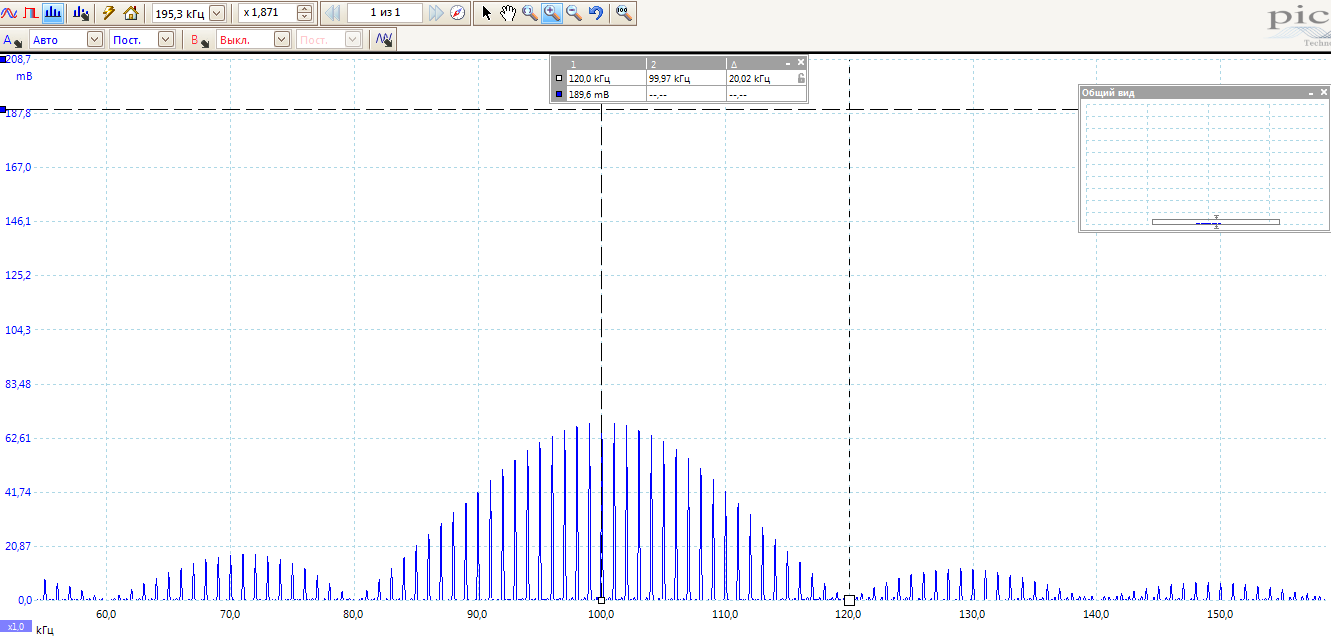
\includegraphics[width=\linewidth]{Graphics/Б_100_1_5.PNG}
  \caption{График 14. $\nu_0 = 100$ кГц, $T = 1$ мс, $N = 5$.}
\end{minipage}
\hfill
\begin{minipage}{0.48\textwidth}
  \centering
  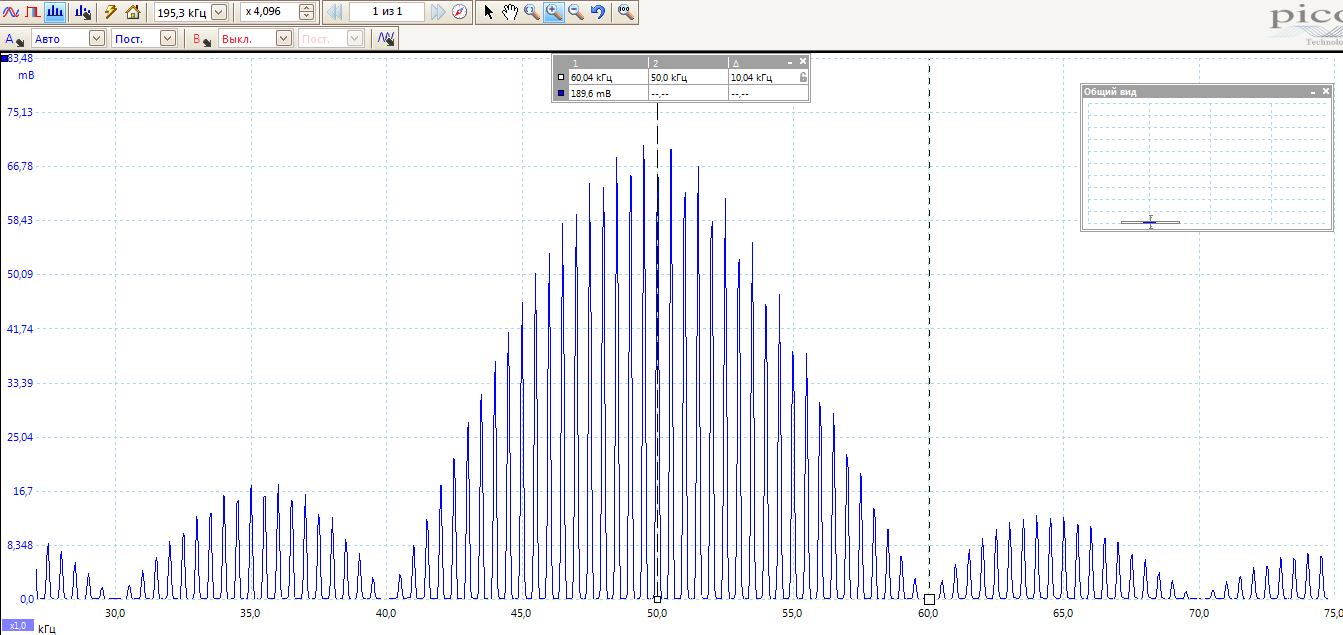
\includegraphics[width=\linewidth]{Graphics/Б_50_2_5.PNG}
  \caption{График 15. $\nu_0 = 50$ кГц, $T = 2$ мс, $N = 5$.}
\end{minipage}

\vspace{1em}

% Строка 4 (один график — можно центрировать)
\begin{minipage}{0.48\textwidth}
  \centering
  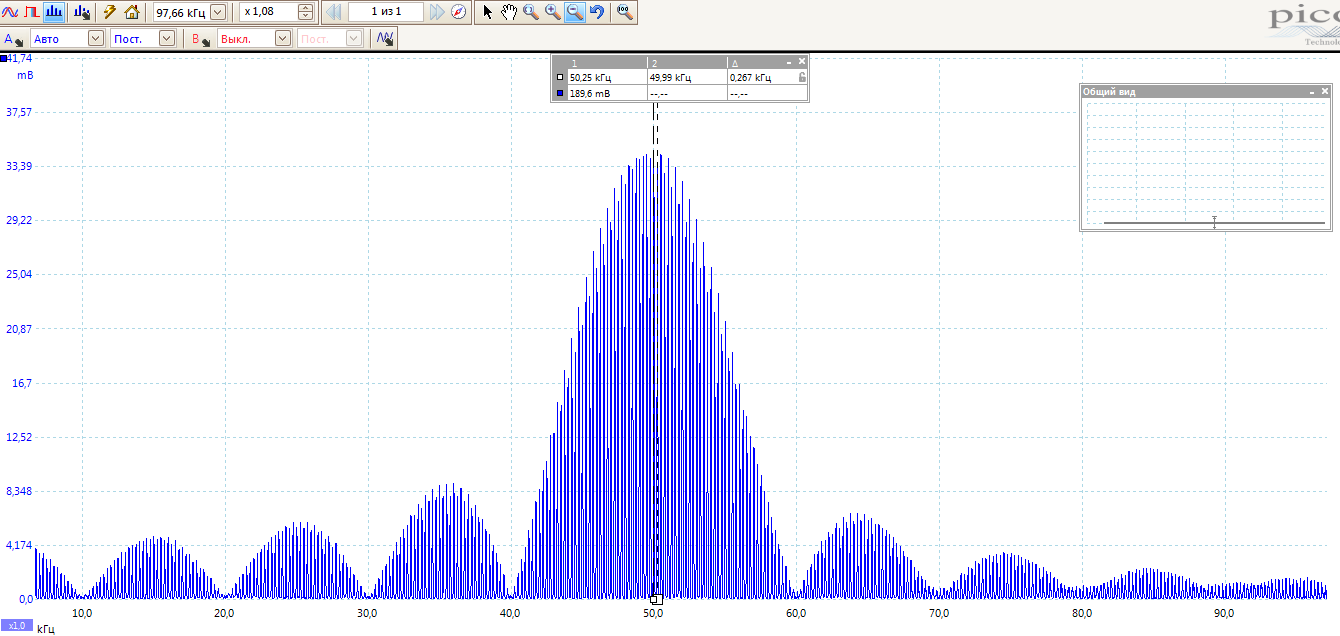
\includegraphics[width=\linewidth]{Graphics/Б_50_4_5.PNG}
  \caption{График 16. $\nu_0 = 50$ кГц, $T = 4$ мс, $N = 5$.}
\end{minipage}

\end{figure}

\clearpage
\begin{table}[h!]
    \centering
    \begin{tabular}{|c|c|c|c|c|c|c|}
        \hline
        № & $\nu_0,\ \text{кГц}$ & $T,\ \text{мкс}$ & $N$ & $\nu_{\text{ц}},\ \text{кГц}$ & $\Delta\nu,\ \text{кГц}$ & $\delta\nu,\ \text{кГц}$ \\
        \hline
        1 & 50 & 1 & 5 & 50{,}02 & 9{,}943 & 0{,}987 \\
        \hline
        2 & 75 & 1 & 5 & 74{,}02 & 10{,}01 & 0{,}987 \\
        \hline
        3 & 100 & 1 & 5 & 99{,}97 & 10{,}02 & 1{,}034 \\
        \hline
        4 & 50 & 2 & 5 & 50{,}00 & 10{,}04 & 0{,}498 \\
        \hline
        5 & 50 & 4 & 5 & 49{,}49 & 10{,}05 & 0{,}267 \\
        \hline
        6 & 50 & 1 & 10 & 49{,}99 & 5{,}017 & 0{,}945 \\
        \hline
        7 & 50 & 1 & 2 & 49{,}99 & 24{,}87 & 1{,}021 \\
        \hline
    \end{tabular}
    \caption{Таблица 4. Результаты измерений центральной частоты $\nu_{\text{ц}}$, ширины спектра $\Delta\nu$ и расстояния между гармониками $\delta\nu$ при различных значениях несущей частоты $\nu_0$, периода $T$ и числа импульсов $N$.}
    \label{tab:frequency_analysis}
\end{table}

Как мы видим, с ростом $N$ спектр "сжимается" к центру (ширина спектра уменьшается), с ростом $\nu_0$ форма спектра не меняется, но центр смещается на несущую частоту, с ростом $T$ уменьшается расстояние между пиками. Наблюдаемое смещение спектра при изменении несущей частоты $\nu_0$ является прямым следствием теоремы о смещении в преобразовании Фурье. Умножение сигнала на гармоническую функцию $\sin(2\pi\nu_0t)$ эквивалентно сдвигу его спектра на $\pm \nu_0$. Экспериментально это проявляется в том, что центр спектра перемещается вместе с изменением $\nu_0$, сохраняя форму и ширину. Это подтверждает справедливость теоремы и позволяет использовать её для анализа модулированных сигналов.

\subsection{Г. Исследование спектра амплитудно-модулированного сигнала}
\item Установим режим модулированного по амплитуде синусоидального сигнала с рекомендованными параметрами: частота несущей $\nu_0 = 50$ кГц, частота модуляции $\nu_{\text{мод}} = 2$ кГц, глубина модуляции $m = 0,5$.\\
С помощью осциллографа (в режиме курсорных измерений) измерим максимальную $A_{max}$ и минимальную $A_{min}$ амплитуды сигнала. $A_{max} = 1,476$ В, $A_{min} = 0,4847$ В, $m = \frac{A_{max} - A_{min}}{A_{max} + A_{min}} = 0,506$, что довольно близко к выставленной глубине 0,5.
\item Изменяя несущую частоту и частоту модуляции, будем измерять частоты центральной и боковой гармоник.

\begin{figure}[h!]
\centering

% Строка 1
\begin{minipage}{0.48\textwidth}
  \centering
  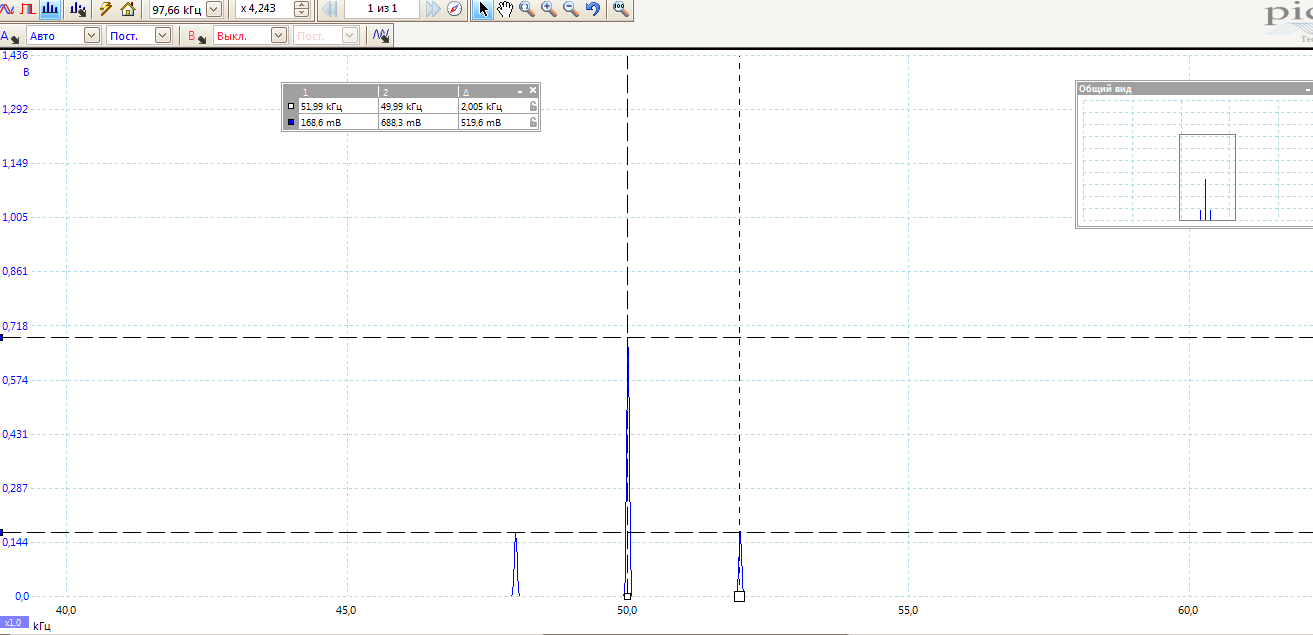
\includegraphics[width=\linewidth]{Graphics/Г_50_2_50.PNG}
  \caption{График 17. $\nu_0 = 50$ кГц, $\nu_{\text{мод}} = 2$ кГц.}
\end{minipage}
\hfill
\begin{minipage}{0.48\textwidth}
  \centering
  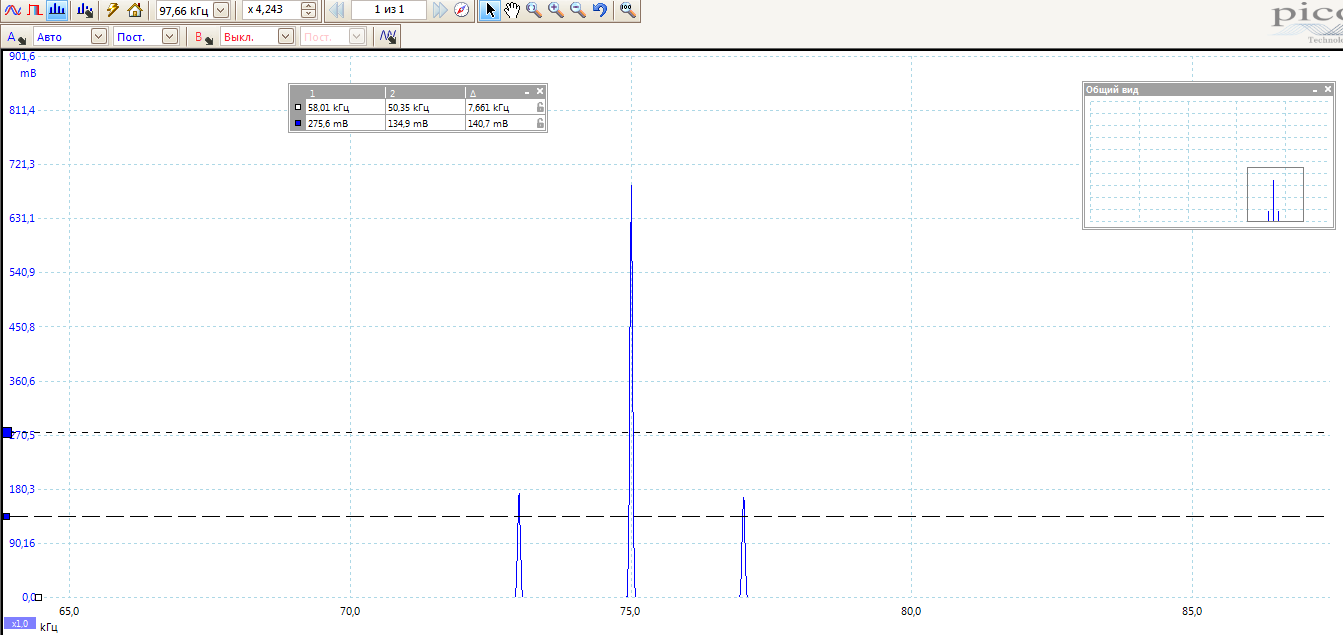
\includegraphics[width=\linewidth]{Graphics/Г_75_2_50.PNG}
  \caption{График 18. $\nu_0 = 75$ кГц, $\nu_{\text{мод}} = 2$ кГц.}
\end{minipage}

\vspace{1em} % Отступ между строками

% Строка 2
\begin{minipage}{0.48\textwidth}
  \centering
  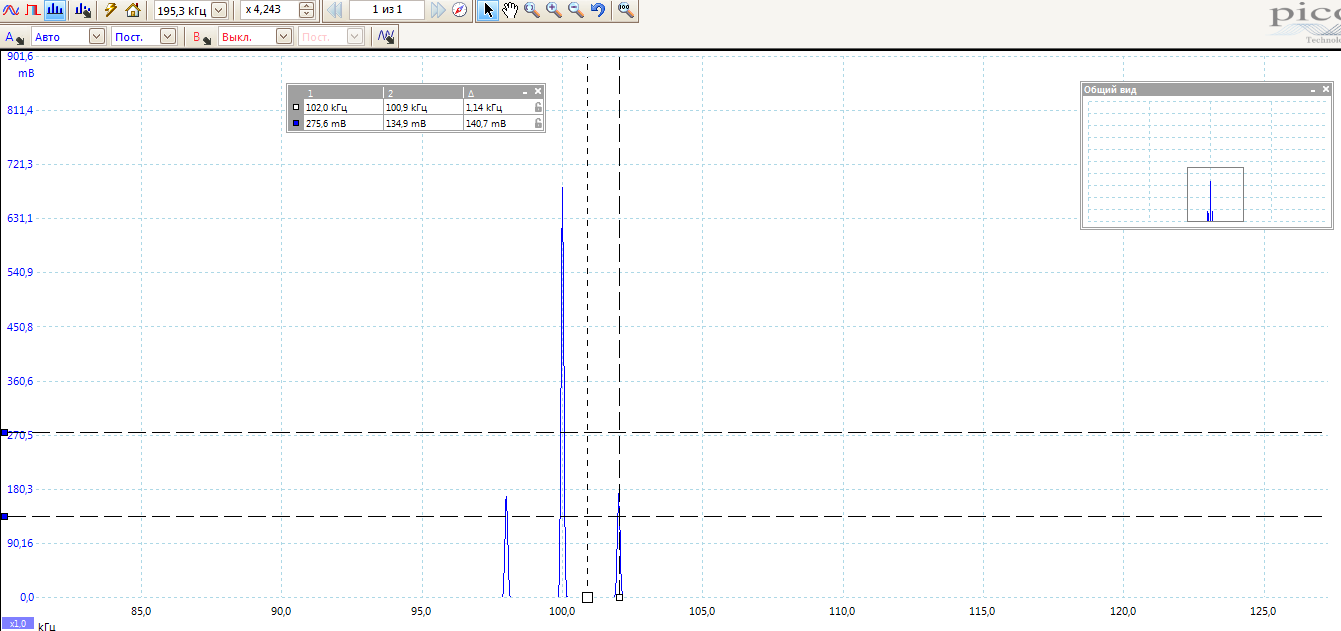
\includegraphics[width=\linewidth]{Graphics/Г_100_2_50.PNG}
  \caption{График 19. $\nu_0 = 100$ кГц, $\nu_{\text{мод}} = 2$ кГц.}
\end{minipage}
\hfill
\begin{minipage}{0.48\textwidth}
  \centering
  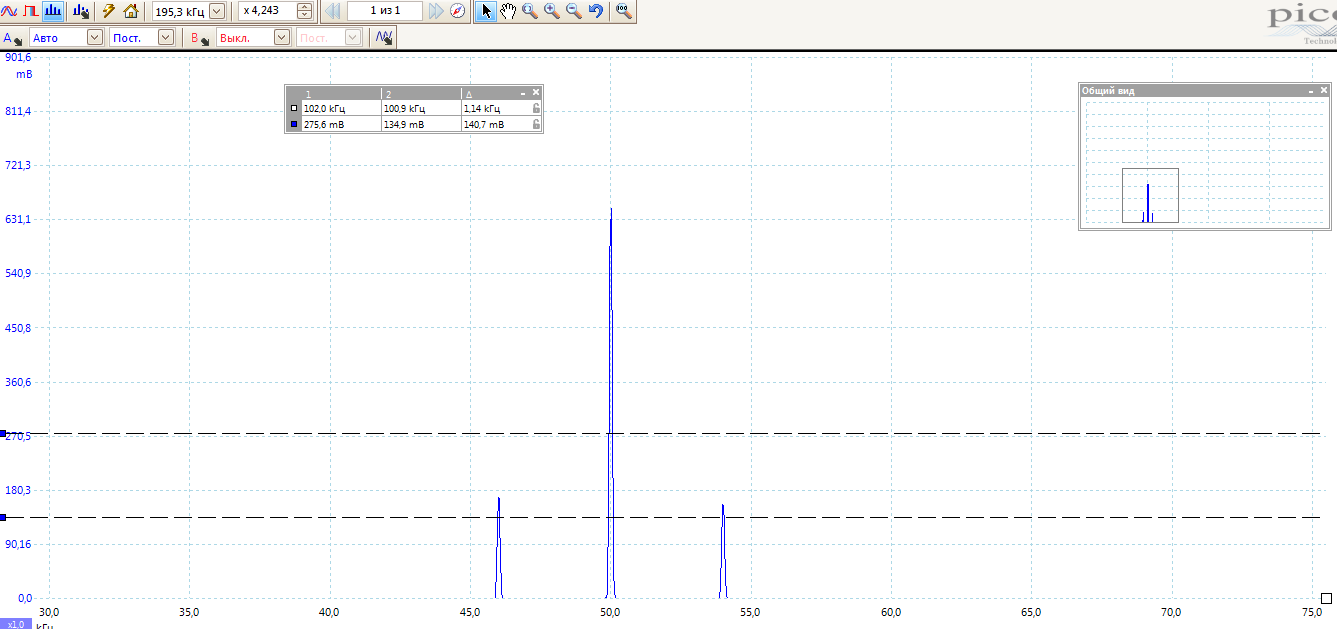
\includegraphics[width=\linewidth]{Graphics/Г_50_4_50.PNG}
  \caption{График 20. $\nu_0 = 100$ кГц, $\nu_{\text{мод}} = 4$ кГц.}
\end{minipage}

\vspace{1em}
\end{figure}
\clearpage
\begin{figure}[h!]
\centering
% Строка 4 (один график — можно центрировать)
\begin{minipage}{0.48\textwidth}
  \centering
  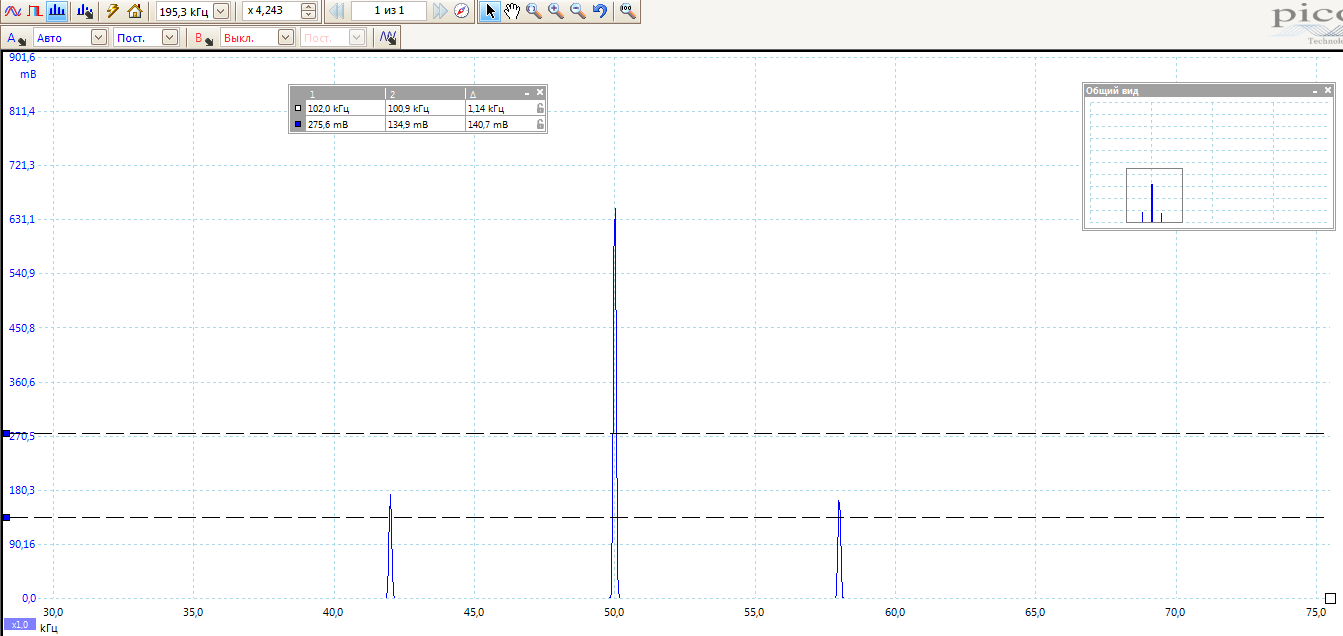
\includegraphics[width=\linewidth]{Graphics/Г_50_8_50.PNG}
  \caption{График 21. $\nu_0 = 100$ кГц, $\nu_{\text{мод}} = 8$ кГц.}
\end{minipage}

\end{figure}

\begin{table}[h!]
    \centering
    \begin{tabular}{|c|c|c|c|c|c|}
        \hline
        № & $\nu_0,\ \text{кГц}$ & $\nu_{\text{мод}},\ \text{кГц}$ & $\nu_{\text{осн}},\ \text{кГц}$ & $\nu_{\text{бок}},\ \text{кГц}$ & $\nu_{\text{мод}}^{\text{эксп}},\ \text{кГц}$ \\
        \hline
        1 & 50 & 2 & 49{,}98 & 51{,}99 & 2{,}005 \\
        \hline
        2 & 75 & 2 & 75{,}00 & 77{,}01 & 2{,}013 \\
        \hline
        3 & 100 & 2 & 100{,}00 & 102{,}00 & 1{,}996 \\
        \hline
        4 & 50 & 4 & 50{,}01 & 53{,}98 & 3{,}973 \\
        \hline
        5 & 50 & 8 & 50{,}01 & 58{,}01 & 8{,}00 \\
        \hline
    \end{tabular}
    \caption{Таблица 5. Значения несущей частоты $\nu_0$, частоты модуляции $\nu_{\text{мод}}$, основной частоты $\nu_{\text{осн}}$, боковой частоты $\nu_{\text{бок}}$ и экспериментальной частоты модуляции $\nu_{\text{мод}}^{\text{эксп}}$}
    \label{tab:modulation_frequencies}
\end{table}


На основе графиков можно сделать вывод о том, что с увеличением несущей частоты смещается основная частота, с увеличением частоты модуляции увеличивается расстояние между гармониками.

\item Изменяя на генераторе глубину модуляции $m$ в диапазоне от 10\% до 100\% будем измерять отношение амплитуд боковой и основной
спектральных линий $\frac{a_{\text{бок}}}{a_{\text{осн}}}$.

\begin{table}[h!]
    \centering
    \begin{tabular}{|c|c|c|c|c|c|c|c|}
        \hline
        $m,\ \%$ & 10 & 20 & 40 & 50 & 60 & 80 & 100 \\
        \hline
        $a_{\text{осн}},\ \text{мВ}$ & 688{,}8 & 688{,}8 & 688{,}8 & 688{,}3 & 688{,}8 & 688{,}8 & 688{,}8 \\
        \hline
        $a_{\text{бок}},\ \text{мВ}$ & 33{,}23 & 66{,}56 & 133{,}2 & 168{,}6 & 199{,}9 & 266{,}5 & 337{,}2 \\
        \hline
        $\left( \frac{a_{\text{бок}}}{a_{\text{осн}}} \right)^{\text{эксп}}$ & 0{,}0482 & 0{,}0966 & 0{,}1934 & 0{,}2450 & 0{,}2902 & 0{,}3869 & 0{,}4895 \\
        \hline
        $\left( \frac{a_{\text{бок}}}{a_{\text{осн}}} \right)^{\text{теор}}$ & 0{,}05 & 0{,}1 & 0{,}2 & 0{,}25 & 0{,}3 & 0{,}4 & 0{,}5 \\
        \hline
    \end{tabular}
    \caption{Таблица 6. Зависимость амплитуд боковых и несущей частот от глубины модуляции $m$}
    \label{tab:am_modulation}
\end{table}

По МНК построим прямую $\left( \frac{a_{\text{бок}}}{a_{\text{осн}}} \right) (m)$.
\clearpage
\begin{figure}[h]
        \center{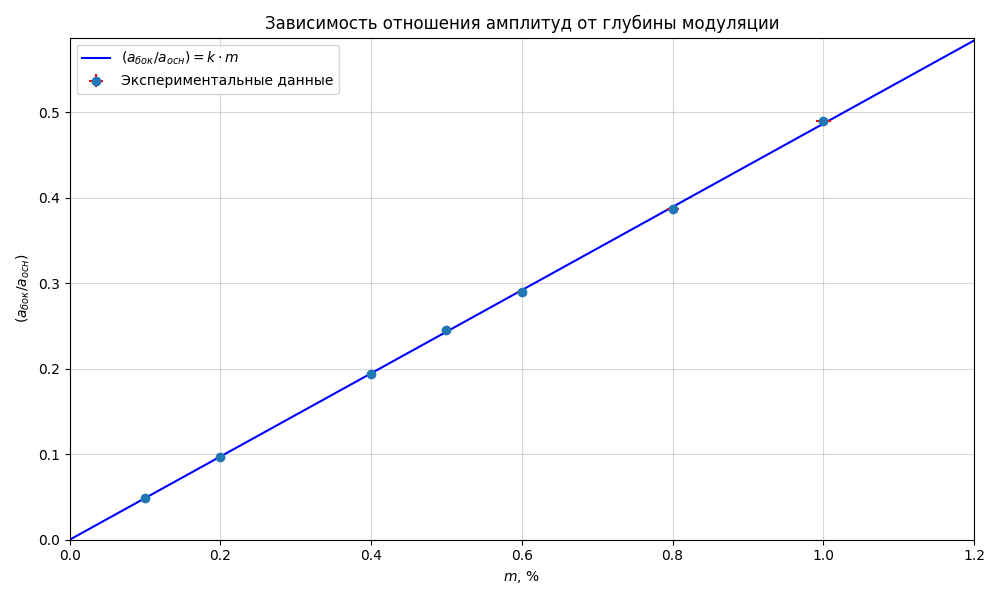
\includegraphics[width=1\textwidth]{Graphics/a_ratio_vs_m_plot_D.png}}
        \caption{График 22. Зависимость отношения боковой амплитуды к основной от глубины модуляции.}
\end{figure}
Наклон прямой $k = 0,4867 \pm 0,0017$ ($\varepsilon_k = 0,5 \%$). Данный результат говорит о том, что соотношение $\frac{a_{\text{бок}}}{a_{\text{осн}}}  = \frac{m}{2}$ выплоняется с хорошей точностью.

\subsection{Д. Наблюдение спектра сигнала, модулированного по фазе}
\item Установим режим модулированного по фазе синусоидального сигнала с рекомендованными параметрами: частота несущей $\nu_0 = 50$ кГц, частота модуляции $\nu_{\text{мод}} = 2$ кГц, максимальное отклонение (глубина модуляции) фазы $\varphi_m = 10^\circ$.\\
\item Изменяя несущую частоту, частоту модуляции и глубину модуляции, будем наблюдать за изменением формы спектра.

\begin{figure}[h!]
\centering

% Строка 1
\begin{minipage}{0.48\textwidth}
  \centering
  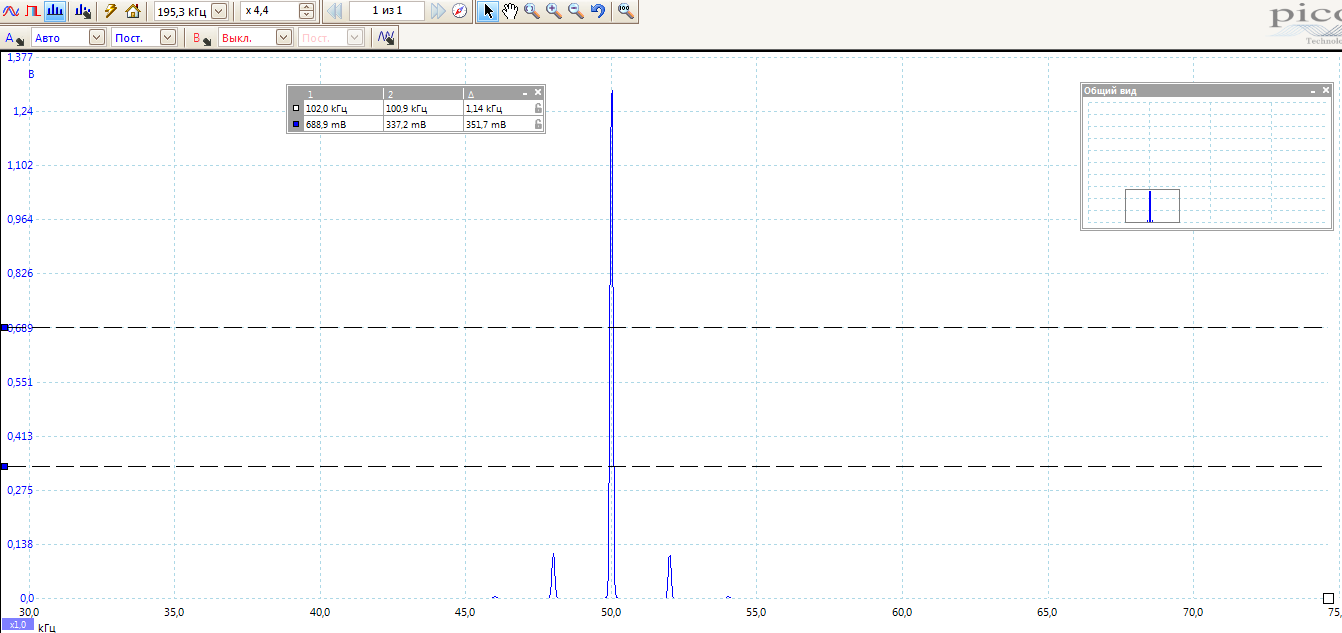
\includegraphics[width=\linewidth]{Graphics/Д_50_2_10.PNG}
  \caption{График 23. $\nu_0 = 50$ кГц, $\nu_{\text{мод}} = 2$ кГц, $\varphi_m = 10^\circ$.}
\end{minipage}
\hfill
\begin{minipage}{0.48\textwidth}
  \centering
  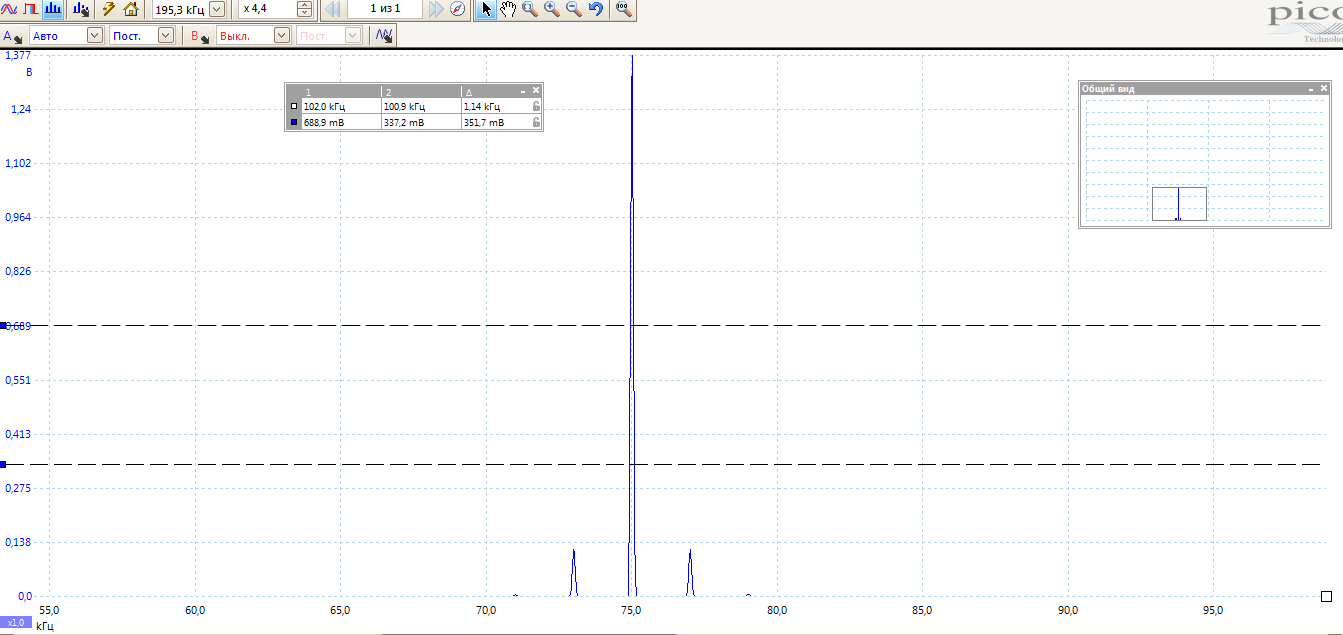
\includegraphics[width=\linewidth]{Graphics/Д_75_2_10.PNG}
  \caption{График 24. $\nu_0 = 75$ кГц, $\nu_{\text{мод}} = 2$ кГц, $\varphi_m = 10^\circ$.}
\end{minipage}

\vspace{1em} % Отступ между строками
\end{figure}
\clearpage
\begin{figure}[h!]
\centering
% Строка 2
\begin{minipage}{0.48\textwidth}
  \centering
  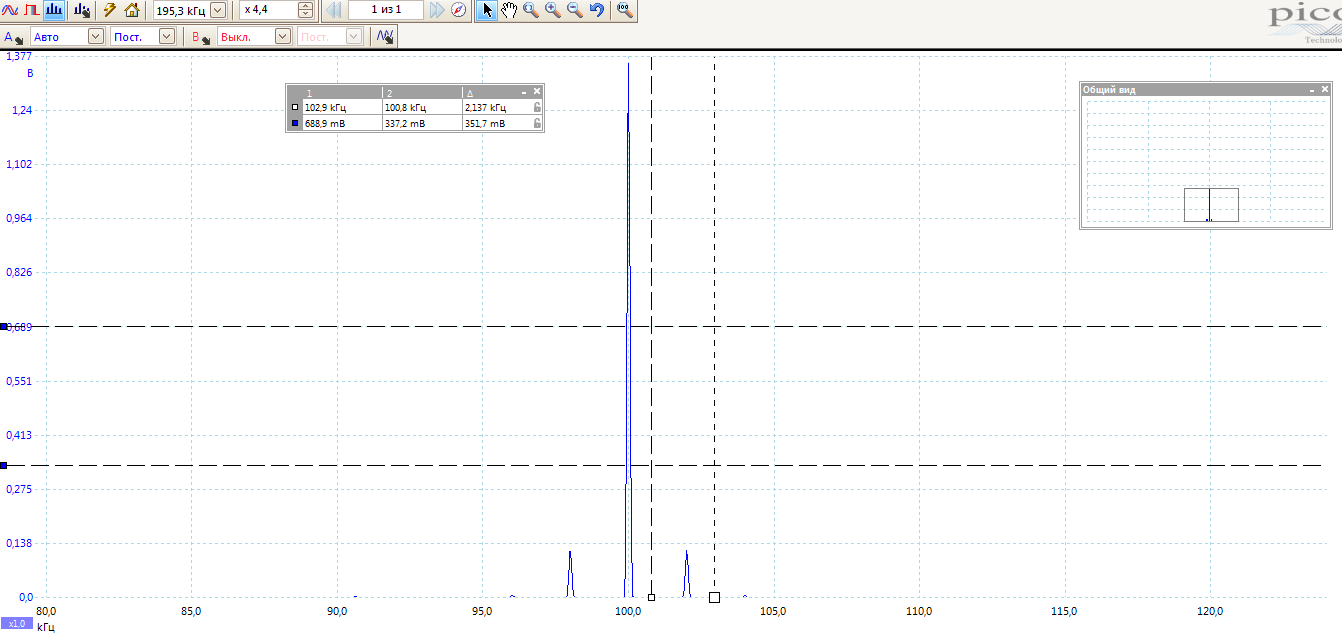
\includegraphics[width=\linewidth]{Graphics/Д_100_2_10.PNG}
  \caption{График 25. $\nu_0 = 100$ кГц, $\nu_{\text{мод}} = 2$ кГц, $\varphi_m = 10^\circ$.}
\end{minipage}
\hfill
\begin{minipage}{0.48\textwidth}
  \centering
  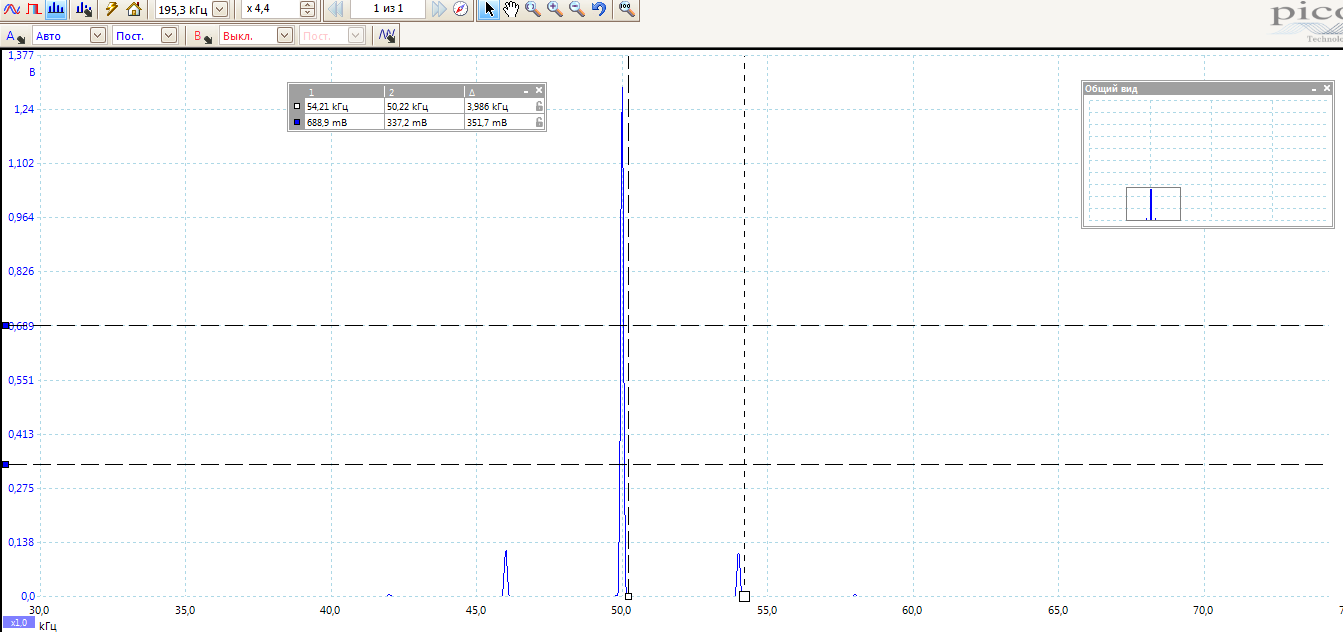
\includegraphics[width=\linewidth]{Graphics/Д_50_4_10.PNG}
  \caption{График 26. $\nu_0 = 50$ кГц, $\nu_{\text{мод}} = 4$ кГц, $\varphi_m = 10^\circ$.}
\end{minipage}

\vspace{1em}

\begin{minipage}{0.48\textwidth}
  \centering
  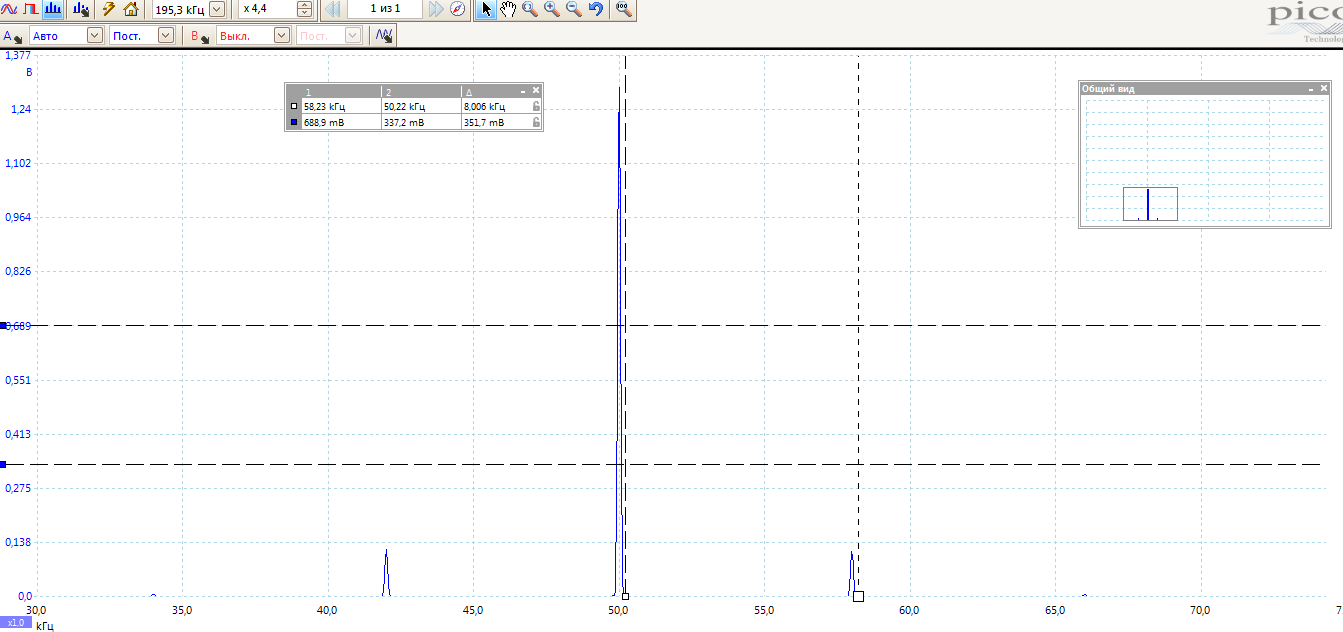
\includegraphics[width=\linewidth]{Graphics/Д_50_8_10.PNG}
  \caption{График 27. $\nu_0 = 50$ кГц, $\nu_{\text{мод}} = 8$ кГц, $\varphi_m = 10^\circ$.}
\end{minipage}
\hfill
\begin{minipage}{0.48\textwidth}
  \centering
  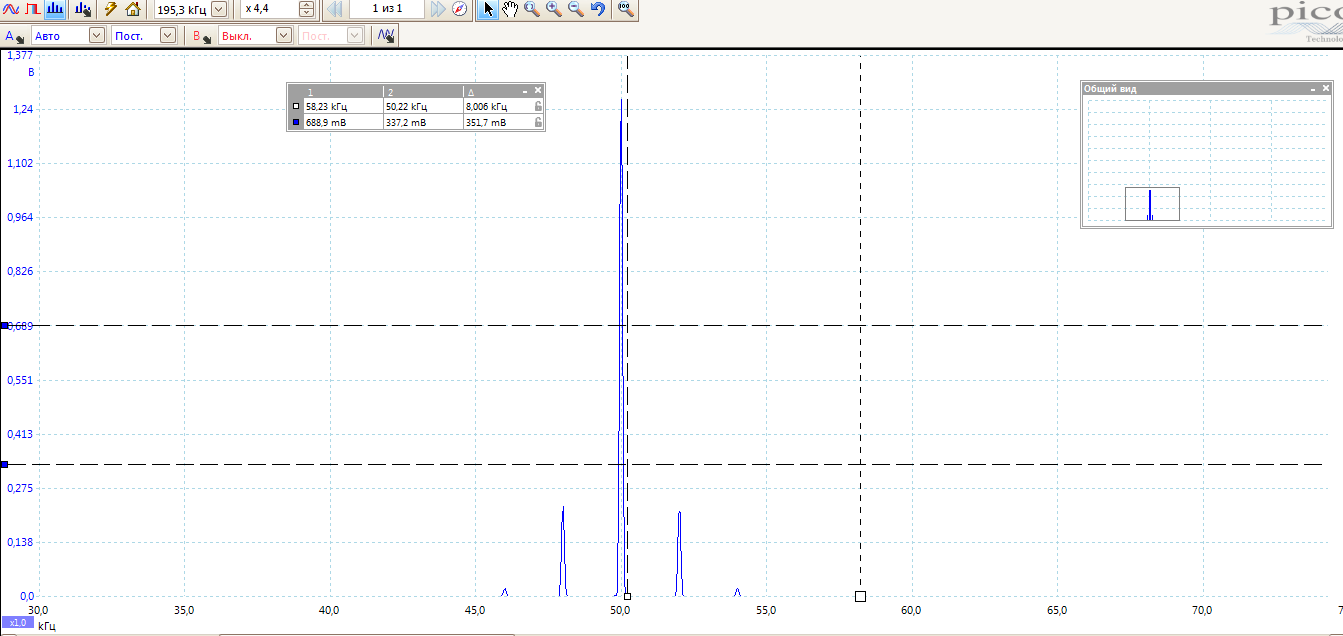
\includegraphics[width=\linewidth]{Graphics/Д_50_2_20.PNG}
  \caption{График 28. $\nu_0 = 50$ кГц, $\nu_{\text{мод}} = 2$ кГц, $\varphi_m = 20^\circ$.}
\end{minipage}

\vspace{1em}

\begin{minipage}{0.48\textwidth}
  \centering
  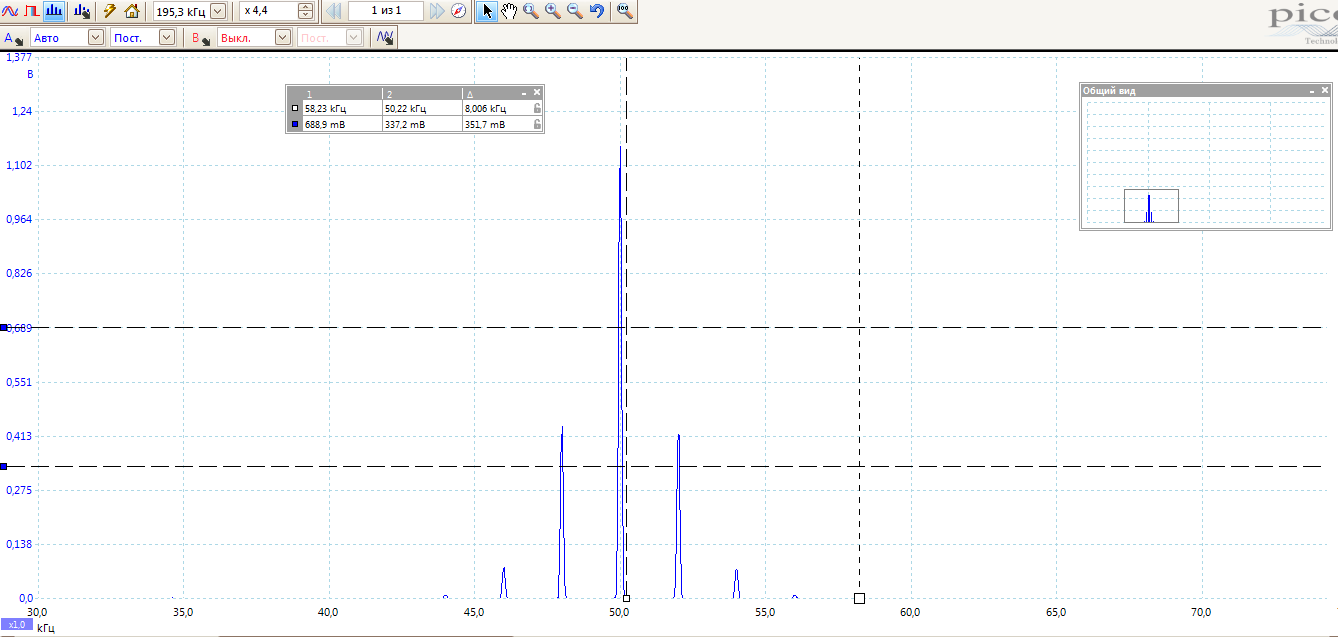
\includegraphics[width=\linewidth]{Graphics/Д_50_2_40.PNG}
  \caption{График 29. $\nu_0 = 50$ кГц, $\nu_{\text{мод}} = 2$ кГц, $\varphi_m = 40^\circ$.}
\end{minipage}
\hfill
\begin{minipage}{0.48\textwidth}
  \centering
  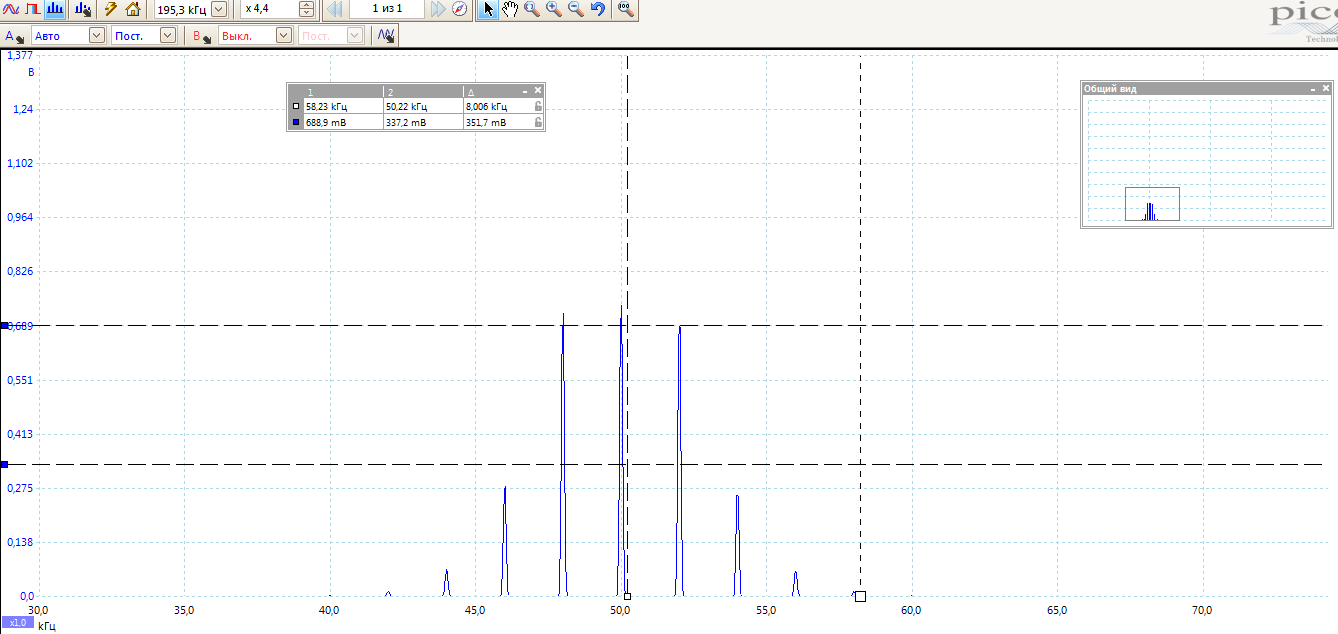
\includegraphics[width=\linewidth]{Graphics/Д_50_2_80.PNG}
  \caption{График 30. $\nu_0 = 50$ кГц, $\nu_{\text{мод}} = 2$ кГц, $\varphi_m = 80^\circ$.}
\end{minipage}

\vspace{1em}

% Строка 4 (один график — можно центрировать)
\begin{minipage}{0.48\textwidth}
  \centering
  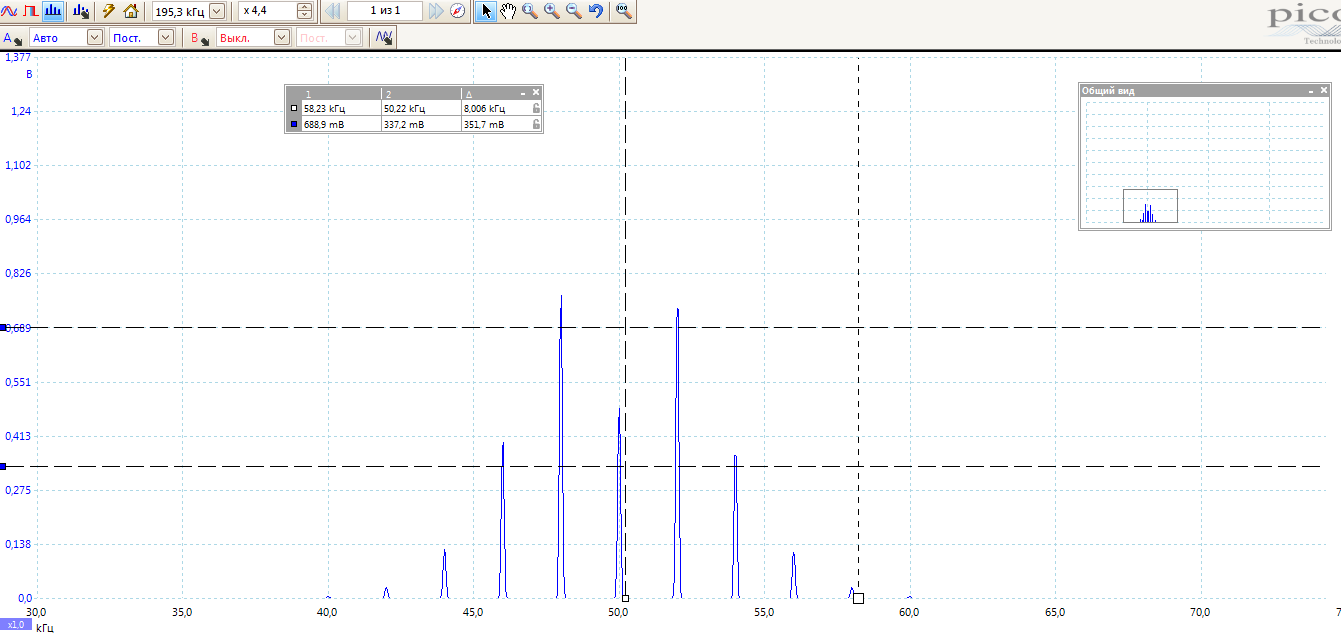
\includegraphics[width=\linewidth]{Graphics/Д_50_2_100.PNG}
  \caption{График 31. $\nu_0 = 50$ кГц, $\nu_{\text{мод}} = 2$ кГц, $\varphi_m = 100^\circ$.}
\end{minipage}

\end{figure}

Как мы видим, с увеличением несущей частоты смещается основная частота, с увеличением частоты модуляции увеличивается расстояние между гармониками. Когда глубина модуляции увеличивается, появляются новые гармоники. Это подтверждает теорию.

\end{enumerate}

\section{Результаты и обсуждения}

\begin{enumerate}
\item В пункте А мы на основе прямоугольных импульсов пронаблюдали изменение спектра от основных параметров (частоты повторения, длительности импульса). Построили а) график  $\Delta \nu(\frac{1}{\tau})$, получили наклон прямой $k = 0,99895 \pm 0,00004$ Гц$\cdot$с ($\varepsilon_k = 0,0037\%$), б) $\delta \nu(\frac{1}{T})$, получили наклон прямой $k = 0,988 \pm 0,001$ Гц$\cdot$с ($\varepsilon_k = 0,11\%$). По ним убедились, что соотношение неопределенностей (4) выполняется с хорошей точностью.
\item В пункте Б исследовали спектр периодической последовательности цугов. По данным таблицы 4 снова убедились в справедливости соотношении неопределенностей и подтвердили теорему о смещении.
\item В пункте Г провели исследование амплитудно-модулированного сигнала. Измерили максимальную и минимальную амплитуды, убедились, что $m^{\text{эксп}} = \frac{A_{max} - A_{min}}{A_{max} + A_{min}} = 0,506$ совпадает с выставленной $m = 0,5$. Увидели, как меняется спектр в зависимости от параметров. По МНК построили прямую $\left( \frac{a_{\text{бок}}}{a_{\text{осн}}} \right) (m)$, наклон прямой получился $k = 0,4867 \pm 0,0017$ ($\varepsilon_k = 0,5 \%$), что очень близко к теоретическому $k = 0,5$.

\item В пункте Д провели наблюдение спектра сигнала, модулированного по фазе.  Подтвердили теорию связанную с изменением спектра при изменении несущей частоты, частоты модуляции  и глубины модуляции.

\end{enumerate}

\section{Выводы}

В данной работе провели исследование спектров прямоугольных импульсов, последовательности цугов, амплитудно-модулированных сигналов, и сигналов, модулированных по фазе. Подтвердили справедливость соотношения неопределенностей, теоремы о смещении.

\end{document}